\chapter{Introducción}

    El diseño de los sistemas de señalamiento es un proceso complejo que involucra, principalmente, tres etapas: el análisis de la red ferroviaria, la detección de zonas de mayor probabilidad de descarrilamientos y colisiones, y la óptima localización de las señales correctas para cada función \cite{Paper_160,Paper_168,Paper_176,Paper_202,Paper_203}. La generación automática del señalamiento es de gran importancia y utilidad para el desarrollo de redes ferroviarias nuevas o para revitalizar redes ferroviarias abandonadas o en desuso. Es relevante incluso en redes ferroviarias que son alteradas debido a la adición, modificación o eliminación de elementos ferroviarios tales como pasos a nivel o plataformas, lo cual implica que el señalamiento debe actualizarse en consecuencia.
    
    En este trabajo presentamos una herramienta capaz de automatizar el diseño del señalamiento y la implementación del sistema de enclavamiento ferroviario para cualquier locación, dado únicamente el diseño de su traza ferroviaria. Se discutirán los detalles del diseño de la herramienta, su arquitectura, casos de uso y aplicaciones en locaciones teóricas y reales.

\section{Topologías ferroviarias}
    \label{sec:topologias}
    Las redes ferroviarias presentan dos piezas fundamentales en su infraestructura: su topología y los elementos ferroviarios que la componen. La topología es el entramado de vías férreas, cuyo diseño busca cumplir una función particular, interconectando diversos elementos ferroviarios. Los elementos ferroviarios pueden ser para determinar la ubicación del tren, para delimitar la circulación de vehículos en cruces ferroviarios, permitir el ascenso y descenso de pasajeros, o para modificar dinámicamente los caminos por los que los trenes circulan, entre otras funciones \cite{Paper_4,Paper_13,Paper_17,Paper_175}

    Muchos de los elementos ferroviarios inciden en la circulación del tren, por lo que el conductor debe ser informado de su estado. Es tarea del señalamiento ferroviario alertar a los conductores ferroviarios de cualquier elemento que pueda representar un peligro, evitando así colisiones con otras formaciones o descarrilamientos en zonas críticas \cite{Paper_168,Paper_176,Paper_202,Paper_203}. 
    
    El señalamiento ferroviario incluye un elemento fundamental: los semáforos ferroviarios, de ahora en adelante denominados "señales". Las señales informan al conductor de la habilitación o denegación de uso de las vías posteriores mediante su color, denominado aspecto. Cada señal puede presentar un único aspecto por vez de un conjunto posible que varía según el país o la región. Los aspectos utilizados en Argentina son el verde (permitido avanzar), amarillo (atención) y rojo (detenerse) \cite{RITO}. Algunas señales pueden no tener el aspecto verde (señales de maniobras de dos aspectos) o incorporar un aspecto extra entre el rojo y el amarillo (señales de cuatro aspectos que incluyen el doble amarillo).
    
    Dos señales consecutivas con la misma dirección y sentido constituyen una ruta ferroviaria \cite{RITO,INTERLOCKING_BASIC,IRSE}. Los operarios ferroviarios solicitan al sistema de enclavamientos las rutas que necesitan de acuerdo con la logística deseada. El sistema de enclavamientos habilitará o denegará las rutas solicitadas en función del estado de los elementos ferroviarios cercanos y de las demás rutas activas. Esta función es vital para el sistema ferroviario y su fin último es permitir la circulación de trenes de forma segura o, de no ser posible, no permitir circulación alguna \cite{Paper_175,Paper_176,INTERLOCKING_BASIC,IRSE}.

	En las siguientes subsecciones, se describen algunas de las topologías ferroviarias más ampliamente utilizadas.
	
    \subsection{Derivación ferroviaria}

Cuando es necesario interconectar dos puntos separados por una distancia de decenas o cientos de kilómetros donde hay poco tráfico ferroviario, resulta económicamente poco conveniente construir vías en ambos sentidos. No obstante, construir una sola vía bidireccional presenta inconvenientes logísticos notorios: una formación que circule entre los puntos A y B excluye a cualquier formación que quiera circular de B a A sin colisionar. %No sería posible utilizar la infraestructura en el sentido opuesto mientras se encuentre ocupada.

La solución mas utilizada emplea islas de enclavamiento a modo de bypass cada cierta cantidad de kilómetros, como se ilustra en la Figura \ref{fig:bypass_1}. Estas islas permiten que las formaciones puedan cruzarse sin riesgo de colisión. La primer formación en llegar a la isla de enclavamientos accede al bypass por la vía superior y espera a que la formación en sentido contrario circule por la vía inferior. Una vez despejado el camino que resta por recorrer, la formación reingresa a la vía principal y retoma su marcha.

    \begin{figure}[h]
        \centering
        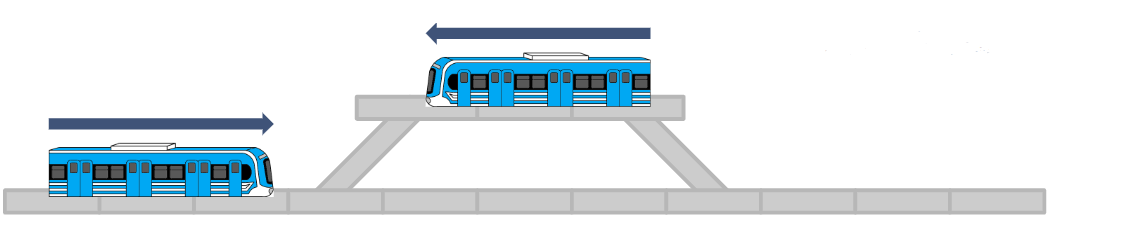
\includegraphics[width=1\textwidth]{Figuras/bypass}
        \centering\caption{Topología de derivación ferroviaria.}
        \label{fig:bypass_1}
    \end{figure}
    
Las topologías de derivación ferroviaria se utilizan principalmente para transportar materias primas entre locaciones rurales a grandes distancias de los puestos. Es deseable tanto una logística óptima, para transportar mas bienes y mas rápido, cómo un sistema seguro que garantice que los bienes lleguen a destino.
    \subsection{Simple}

En entornos urbanos donde las estaciones ferroviarias se encuentran separadas entre sí por unos pocos kilómetros es necesaria una interconectividad mayor. El sistema ferroviario debe satisfacer la demanda de una población mayor y a la vez coexistir con un trazado vehicular mucho mas denso que cruza al trazado ferroviario en varios puntos. En este contexto, una topología simple como la presentada en la Figura \ref{fig:simple_1} es una solución óptima al problema planteado.

    \begin{figure}[h]
        \centering
        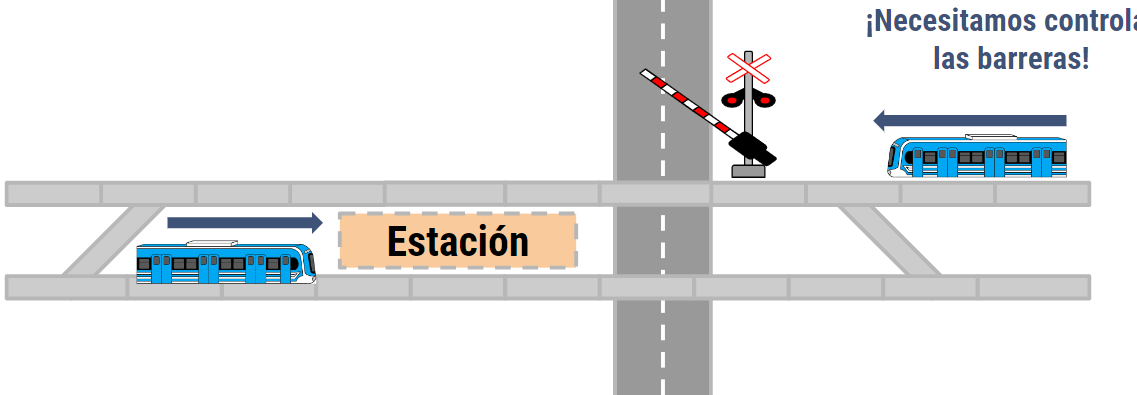
\includegraphics[width=1\textwidth]{Figuras/simple}
        \centering\caption{Topología simple.}
        \label{fig:simple_1}
    \end{figure}

El cruce entre el trazado ferroviario y el trazado vehicular se denomina paso a nivel. El sistema de enclavamientos deberá garantizar que el paso a nivel se encuentre despejado de vehículos y peatones antes de permitir la circulación de trenes sobre el mismo. Esto se logra mediante el uso de una barrera ferroviaria, un mecanismo que mantiene la barrera en alto mientras no se detecten formaciones en las proximidades del paso a nivel.

Las topologías simples suelen contar con dos vías unidireccionales en sentido ascendente y descendente. 
Las vías ascendentes son aquellas por las que las formaciones circulan en la dirección del kilometraje creciente. Mientras que las vías descendentes son aquellas por las que circulan en la dirección del kilometraje decreciente [REF]. El kilómetro cero es la estación principal de la línea ferroviaria, como por ejemplo: Plaza Constitución (Línea Roca), Once de Septiembre (Línea Sarmiento) o Retiro (Línea Mitre y Linea San Martín). Las formaciones pueden cambiar de vía ascendente a descendente, o viceversa, utilizando un cambio ferroviario.
    \subsection{Hub}

A medida que mas líneas ferroviarias coexisten en la misma red se vuelve inevitable que varias líneas compartan la misma estación utilizando diferentes plataformas en paralelo. Con una logística mas flexible, las diferentes líneas incluso pueden utilizar de forma alternada las mismas plataformas y, por lo tanto, las mismas vías principales. Además, es necesario contar con mecanismos para retirar trenes de la red para su mantenimiento y volver a inyectarlos a la red cuando la demanda aumente. Esto se logra por medio de talleres ferroviarios en las inmediaciones de las estaciones que actúan como un hub ferroviario. La topología de hub ferroviario se ilustra en la Figura \ref{fig:hub_1}.

    \begin{figure}[h]
        \centering
        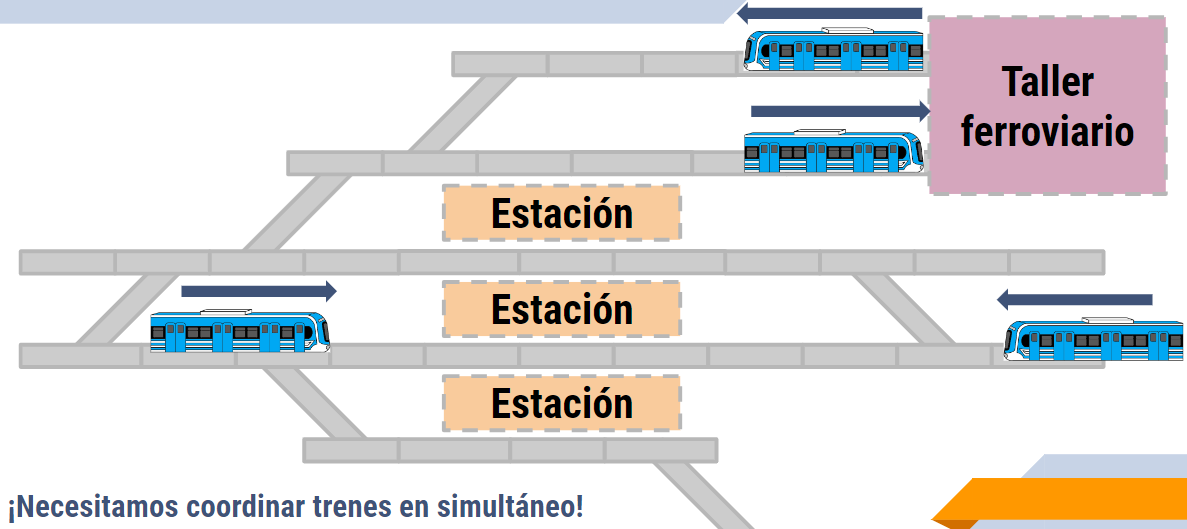
\includegraphics[width=1\textwidth]{Figuras/hub}
        \centering\caption{Topología hub.}
        \label{fig:hub_1}
    \end{figure}
    
Las tareas del sistema de enclavamientos van aumentando en complejidad a medida que se suman nuevos actores. Debe coordinar diversas formaciones de distintas líneas, accediendo a diferentes plataformas, cumpliendo diferentes horarios de arribo y partida. A su vez, debe asegurarse de que las formaciones circulen con seguridad pero sin descuidar la puntualidad. Adicionalmente, debido a que la demanda varía a lo largo del día, deberá tener flexibilidad para inyectar nuevas formaciones a la red o remover las que presenten desperfectos técnicos. Todas estas acciones deben realizarse en simultáneo y en un entorno de alto dinamismo.
    \subsection{Estación Terminal}

Las estaciones terminales presentan una gran cantidad de vías principales y plataformas en paralelo, en las cuales confluyen una o varias líneas ferroviarias. A diferencia de estaciones de tipo hub que pueden presentar finales de vía relativos, las estaciones terminales poseen finales de vía absolutos. Es decir, las formaciones que circulan por la vía descendente deberán detener su marcha completamente antes de llegar al fía de vía, para luego retomar su marcha en sentido contrario, por la vía ascendente. Esta operación puede realizarse de manera inmediata en formaciones con locomotras eléctricas en ambos extremos del tren o con locomotoras diesel luego de varias maniobras que requieren el uso de diversos cambios de vías. En la Figura \ref{fig:terminal_1} se ilustra un ejemplo de una estación terminal.

    \begin{figure}[h]
        \centering
        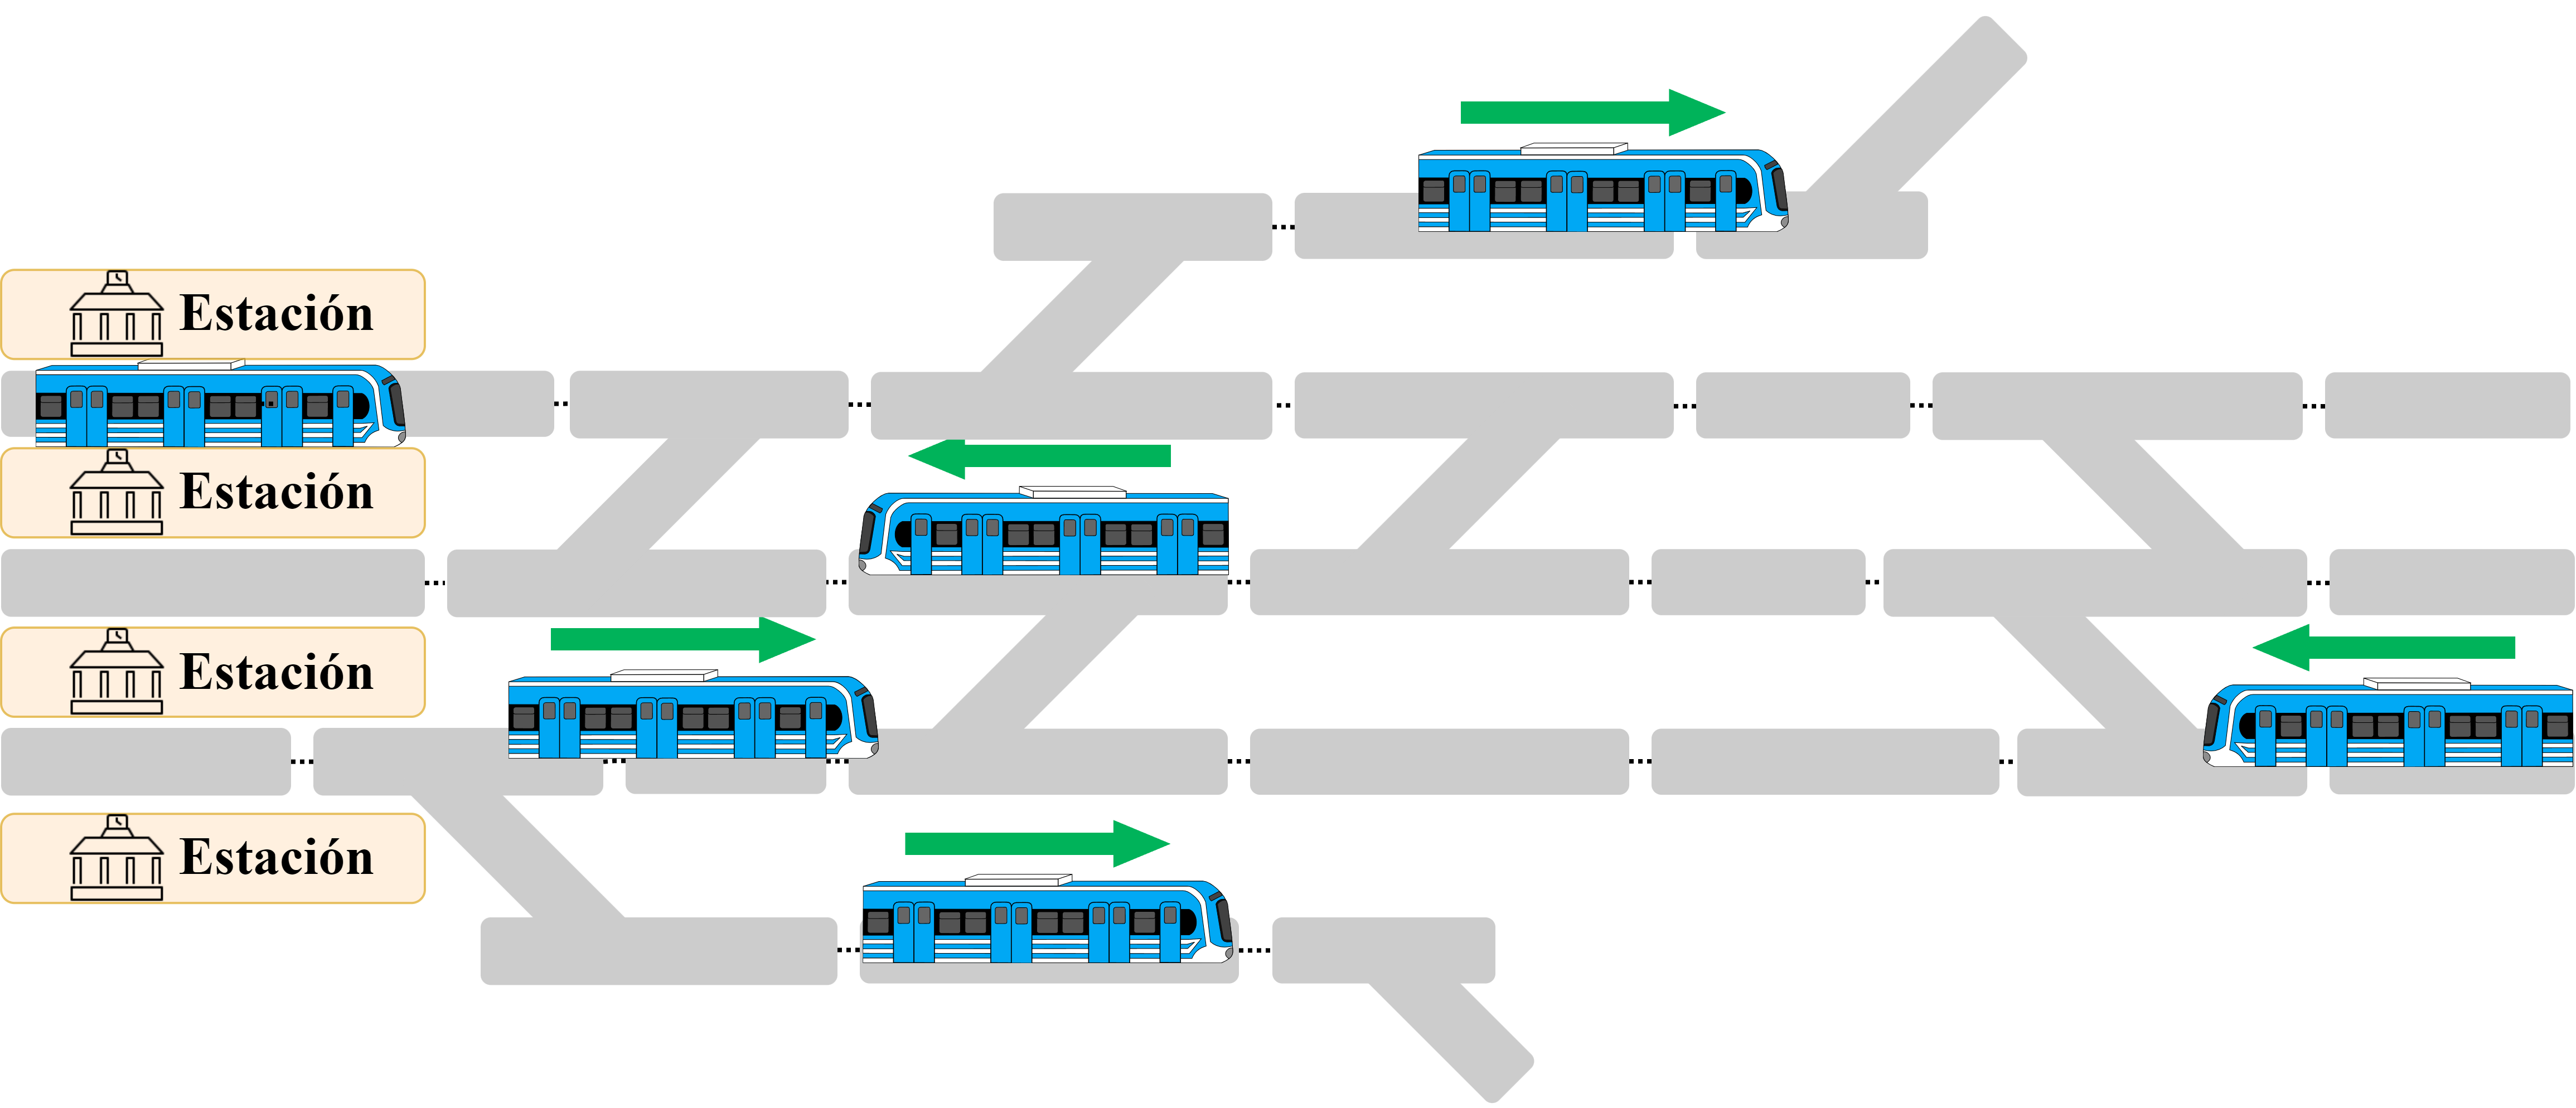
\includegraphics[width=1\textwidth]{Figuras/terminal}
        \centering\caption{Topología terminal.}
        \label{fig:terminal_1}
    \end{figure}

En las estaciones terminales suelen confluir la información en tiempo real de la terminal y las estaciones mas próximas de la línea, o incluso la información en tiempo real de la totalidad de la línea. Esta característica, además de ser la estación de mayor tamaño de la línea, les otorga una jerarquía tal que suelen concentrar parcial o totalmente el control del señalamiento de la red. Las decisiones tomadas en una estación terminal tienen un gran impacto en el sistema de transporte de toda la línea, directa o indirectamente. Estas operaciones deben considerar cientos o miles de estados en simultáneo, por lo que ejecutarlas de forma manual es muy complejo o incluso imposible. Un sistema de enclavamientos moderno, robusto, que pueda garantizar una altísima disponibilidad, mantenibilidad y seguridad es indispensable para llevar a cabo estas tareas.
\section{Principios de señalamiento ferroviario}
    \label{sec:principios}
    
    El proceso de diseño del señalamiento requiere reglas claras y bien definidas sobre cuántas señales colocar, dónde colocar cada señal, bajo que condiciones, de qué tipo deben ser las señales, cómo deben orientarse, etc. Lamentablemente, el criterio utilizado a la hora de definir el señalamiento dista de ser uniforme de nación a nación. La obligatoriedad de ciertas señales, la protección de ciertos elementos, el granularidad de la red o incluso el tener las reglas por escrito son factores que cambian al atravesar las fronteras de cada país. Esto implica, claramente, una barrera enorme al tratar de integrar las redes ferroviarias transnacionales, como en el caso Europeo durante formación de la Unión Europea[REF].
    
    Para la realización de este trabajo se optó por recurrir al Instituto de Ingenieros en Señalamiento Ferroviario (IRSE, por sus siglas en inglés) [IRSE] y a la Junta de Normas y Seguridad de la Industria Ferroviaria (RISSB, por sus siglas en inglés) [RISSB]. Los reglamentos de diseño y definiciones de estas organizaciones son aceptadas por una gran cantidad de empresas del sector ferroviario y autoridades de gran peso. Entre ellas, por la agencia de transporte de Nueva Gales del Sur, en Australia (TfNSW, por sus siglás en inglés) [TfNSW]. De ésta última se recopilaron los siguientes principios de diseño ferroviario:
    
    \begin{itemize}
        \item [($P_1$)] Principio de autoridad: el derecho del tren a circular esta limitada a una pequeña porción de la infraestructura.
        \item [($P_2$)] Principio de claridad: las autoridades otorgadas o negadas no deben ser ambiguas. 
        \item [($P_3$)] Principio de anticipación: los conductores de trenes deben ser advertidos de los peligros cercanos con el suficiente tiempo para reaccionar.
        \item [($P_4$)] Principio de granularidad: las rutas deben ser lo mas cortas posibles.
        \item [($P_5$)] Principio de terminalidad: los conductores de trenes deben ser advertidos cuando se encuentren circulando próximos al final de la red.
        \item [($P_6$)] Principio de infraestructura: los conductores de trenes deben ser advertidos de cualquier infraestructura dinámica o estática próxima.
        \item [($P_7$)] Principio de no bloqueo: se debe evitar en todo momento que los trenes bloqueen el acceso a la infraestructura o ramificaciones a otros tresnes, de ser posible.
    \end{itemize}

    La totalidad del análisis realizado en este proyecto se basa en los principios expuestos. Se puede deducir de los mismos que un sistema de señalamiento debe proteger cada elemento ferroviario ($P_1$,$P_5$,$P_6$), en cada dirección posible ($P_3$,$P_7$). Por lo tanto debemos considerar la posibilidad de que cada tramo de vía puede ser transitado en ambos sentidos ($P_2$,$P_4$) . Esto implica a su vez considerar todas las rutas posibles soportadas por la red ferroviaria, y no solamente las necesarias desde un punto de vista logístico.
\section{Sistemas de enclavamiento}

\subsection{Tipos de sistemas de enclavamiento}
	\label{sec:FPGA}
	
    Los primeros sistemas de enclavamiento implementados fueron mecánicos \cite{Paper_179}. Estos utilizaban palancas, como las que se visualizan en la Figura \ref{fig:enclavamiento_1}, para comandar los cambios de vías y semáforos. Una palanca que habilite una ruta se encuentra bloqueada mecánicamente (enclavada) hasta que todas las palancas que afecten a los elementos ferroviarios correspondientes a esa ruta se encuentre en la posición que garanticen que la ruta es segura. De la misma manera, una vez habilitada una ruta, no es posible mecánicamente mover una palanca que habilite una ruta contraria y, por lo tanto, lleve a dos formaciones a colisionar frontal o lateralmente.
    
        \begin{figure}[H]
            \centering
            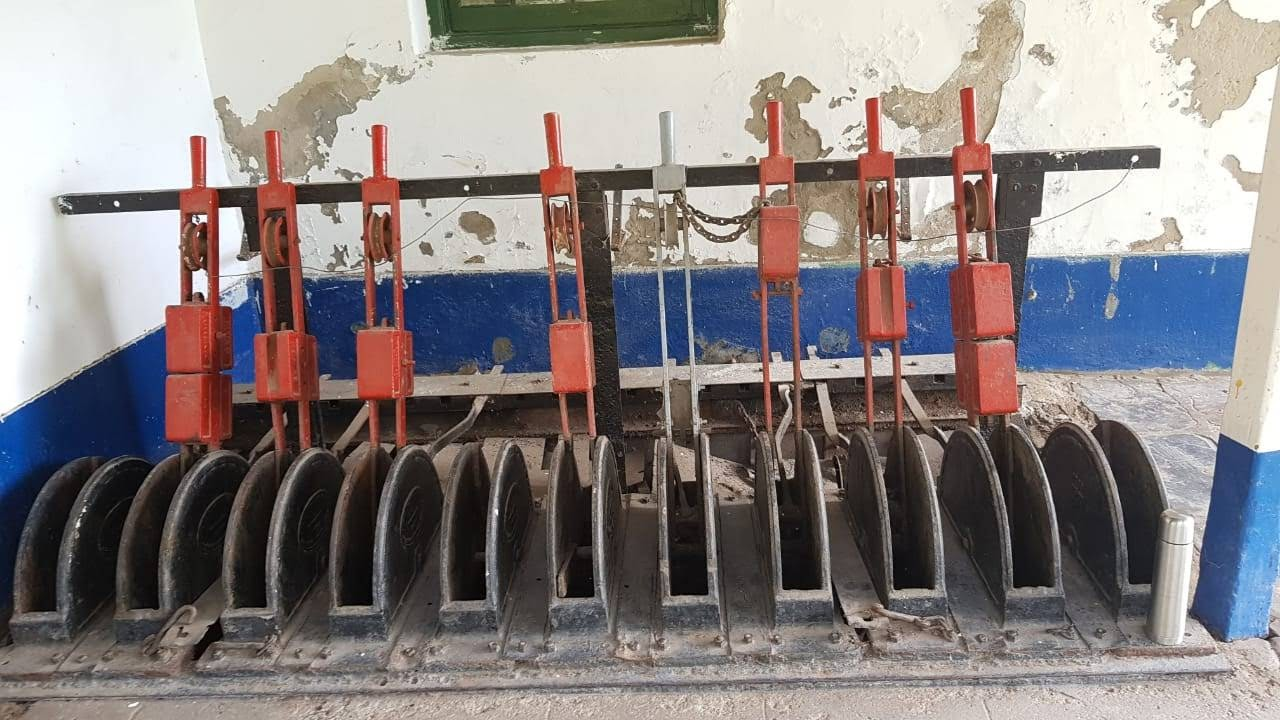
\includegraphics[width=1\textwidth]{Figuras/palancas.jpg}
            \centering\caption{Sistema de enclavamiento mecánico basado en palancas.}
            \label{fig:enclavamiento_1}
        \end{figure}

    Aunque hoy en día las tecnologías mas modernas ya no utilizan bloqueos mecánicos, se sigue utilizando el término \textit{enclavamiento}. En lugar de palancas y mecanismos de bloqueo, se utilizan circuitos lógicos, tanto eléctricos como electrónicos, y lógica programable que permitan garantizar el mismo objetivo: verificar condiciones previo a autorizar una ruta y prohibir la habilitación de rutas conflictivas con las actualmente activas.

    A comienzos del siglo XX se empezaron a utilizar sistemas de enclavamiento electromecánicos en entornos urbanos y semi-urbanos \cite{Paper_1}. Hoy en día este sistema es de los mas utilizado en muchos países \cite{Paper_179}, sobretodo en áreas rurales donde los sistemas tardan mas en actualizarse en comparación con las áreas urbanas. Un sistema de enclavamiento electromecánico se basa en relés (Figura \ref{fig:enclavamiento_2}) y circuitos de vía. Los circuitos eléctricos implementados con relés determinan la lógica del enclavamiento y son necesarios unas pocas decenas de relés para operar una derivación ferroviaria, pero cientos a miles para una estación terminal de gran tamaño \cite{Paper_199}.

    \begin{figure}[H]
        \centering
        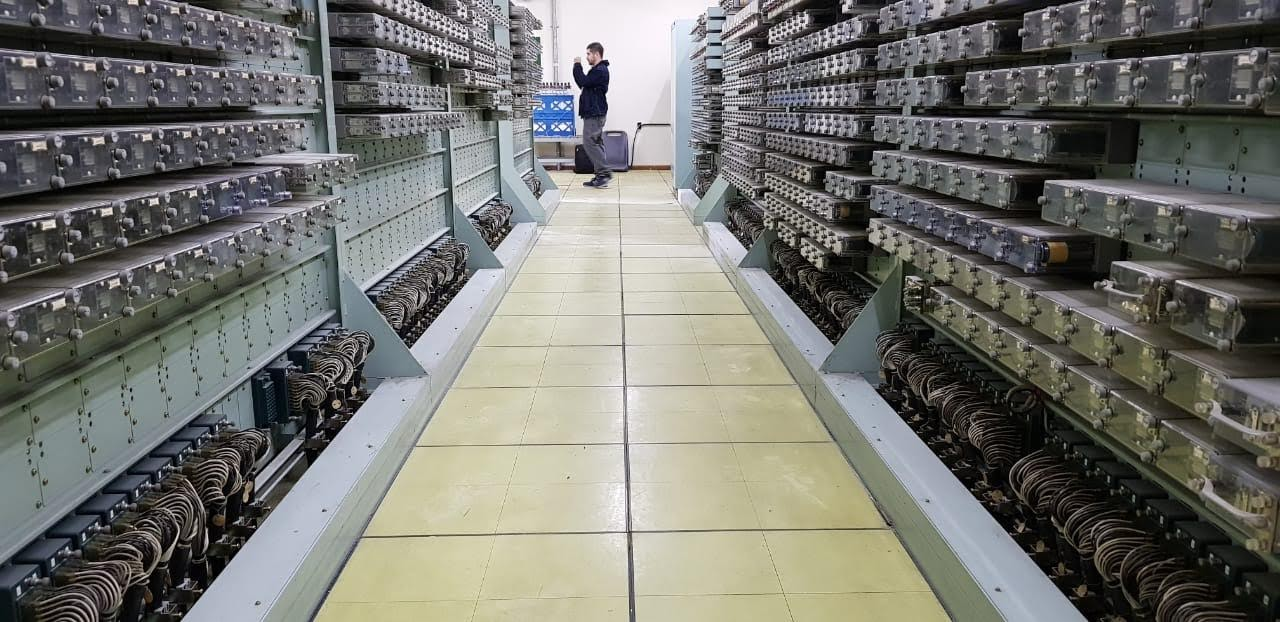
\includegraphics[width=1\textwidth]{Figuras/relees.jpg}
        \centering\caption{Sistema de enclavamiento electromecánico basado en relés.}
        \label{fig:enclavamiento_2}
    \end{figure} 
    
    Los sistemas de enclavamiento electromecánicos son comandados por un operario mediante un panel de control (Figura \ref{fig:enclavamiento_3}). El operario solicita al sistema de enclavamiento las rutas que el conductor ferroviario necesita para transitar por la vía. El sistema de enclavamiento solamente habilitará las rutas seguras, indicando al conductor que puede avanzar mediante un semáforo de aspecto verde o amarillo. En caso de que la ruta no sea habilitada, el sistema \textit{enclavará} los estados de los elementos ferroviarios pertenecientes a esa ruta y le indicará al conductor que no puede continuar su recorrido con un semáforo de aspecto rojo. El operario puede volver a pedir la ruta si las condiciones del sistema cambiaron.
    
    \begin{figure}[H]
        \centering
        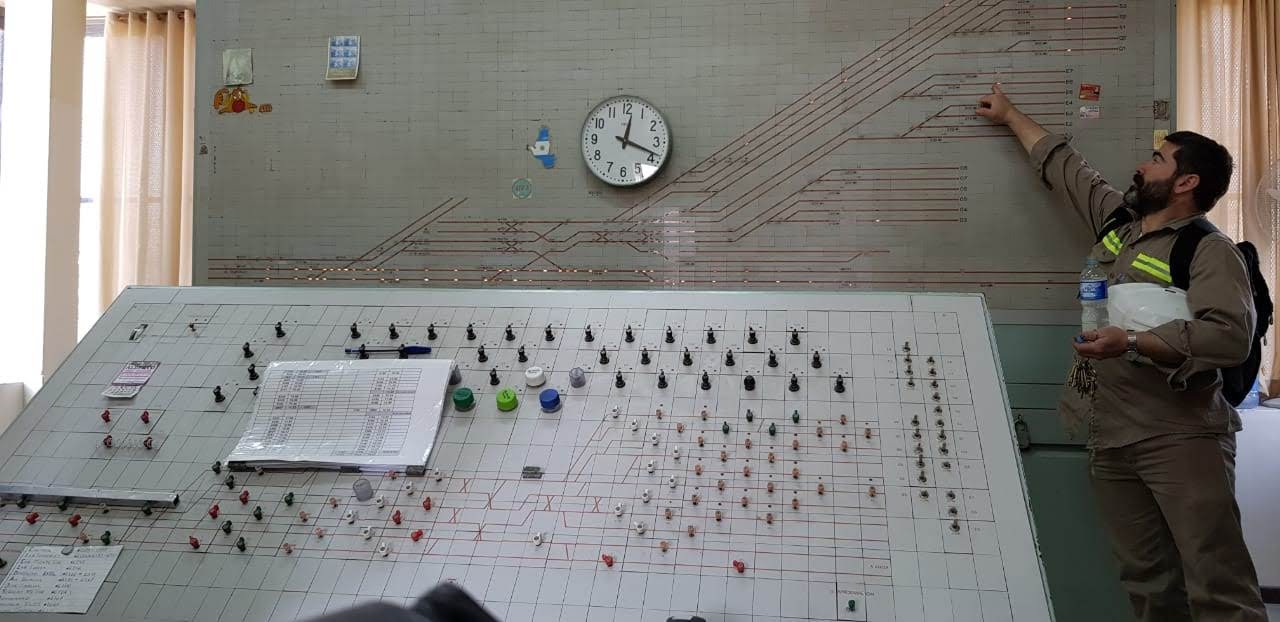
\includegraphics[width=1\textwidth]{Figuras/llavallol.jpg}
        \centering\caption{Panel de control central de un sistema de enclavamientos.}
        \label{fig:enclavamiento_3}
    \end{figure}

    En la actualidad, los sistemas de enclavamiento mas modernos son electrónicos, basados en microprocesadores, PLCs (Controlador Lógico Programable, del inglés Programmable Logic Controllers), o FPGAs (Matriz de puerta programable en campo, del inglés Field-programmable Gate Array) \cite{Paper_3,Paper_8,Paper_16,Paper_18,Paper_22,Paper_24,Paper_25,Paper_28,Paper_31,Paper_34,Paper_35,Paper_36,Paper_119,Paper_137}. Estas tecnologías presentan la ventaja de ser reprogramables una vez instaladas, lo que aporta flexibilidad al diseño, escalabilidad y robustez \cite{Paper_38,Paper_46,Paper_47,Paper_105,Paper_118,Paper_124,Paper_128,Paper_130,Paper_131,Paper_133,Paper_135,Paper_204}. Además, ocupan mucho menos espacio que su contraparte electromecánica, reduciendo los costes de infraestructura, consumo eléctrico y mantenimiento. Se utilizan principalmente en redes de procesamiento distribuido, debido a su integración de forma nativa con protocolos de comunicación industrial diseñados para entornos ferroviarios \cite{Paper_125,Paper_37,Paper_41}. Adicionalmente, los sistemas electrónicos pueden ser fácilmente auditados y redundados, para aumentar su fiabilidad y comprobar su nivel de seguridad \cite{Paper_23,Paper_29,Paper_43,Paper_49,Paper_97,Paper_98,Paper_132,Paper_140}.
\subsection{Tablas de enclavamientos}
	\label{sec:tablas}
	Históricamente, tanto los enclavamientos mecánicos como los electromecánicos se han definido mediante tablas de enclavamientos \cite{INTERLOCKING_BASIC,RITO,IRSE,Paper_204,Paper_205}, las cuales luego pueden ser usadas para definir la logística de la red. Es por eso que el personal técnico está muy capacitado tanto en la lectura de la tabla como en su elaboración.
	
	Cada ruta es definida junto con los elementos ferroviarios que la condicionan y los estados que deben tener los mismos para que la ruta sea habilitada. Además, se explicita cada una de las rutas que entrarían en conflicto con la ruta en cuestión. A modo de ejemplo se presenta en la Figura \ref{fig:funcional_1} como se realiza la asignación de rutas en un cambio de vías.
	
	\begin{figure}[h]
		\centering
		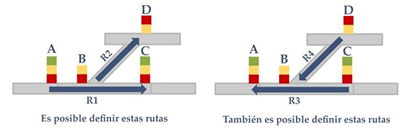
\includegraphics[width=1\textwidth]{Figuras/rutas.PNG}
		\centering\caption{Ejemplo de asignación de rutas.}
		\label{fig:funcional_1}
	\end{figure}
	
	Si el trazado de vías fuese utilizado para circular únicamente de izquierda a derecha, podemos definir únicamente dos rutas. La primera será la ruta R1, desde la señal A hasta la señal C. La segunda ruta R2 se define desde la señal B hasta la señal D, utilizando el cambio de vía a reverso. Ambas rutas quedan definidas en la Tabla \ref{Tab:funcional_2}.
	
	\begin{table}[!h]
		{
			\caption{Tabla de enclavamientos (rutas de izquierda a derecha).}
			\label{Tab:funcional_2}
			\centering
			%\small
			%\centering
			\begin{center}
				\resizebox{0.75\textwidth}{!}{
					\begin{tabular}{ c c c }
						\hline	
						Ruta & Señal de entrada & Señal de salida \\	
						\hline
						R$_1$ & Señal$_{\text{A}}$ & Señal$_{\text{C}}$ \\
						R$_2$ & Señal$_{\text{B}}$ & Señal$_{\text{D}}$ \\
						%\hline
					\end{tabular}
				}
			\end{center}
		}    
	\end{table}
	
	De forma análoga, podríamos analizar el mismo trazado de vías asumiendo que las formaciones circularán estrictamente de derecha a izquierda, definiendo otro nuevo conjunto de rutas. Sumando así las rutas R3 y R4 como se visualiza en la Tabla \ref{Tab:funcional_3}
	
	\begin{table}[!h]
		{
			\caption{Tabla de enclavamientos (rutas de derecha a izquierda).}
			\label{Tab:funcional_3}
			\centering
			%\small
			%\centering
			\begin{center}
				\resizebox{0.75\textwidth}{!}{
					\begin{tabular}{ c c c }
						\hline	
						Ruta & Señal de entrada & Señal de salida \\	
						\hline
						R$_3$ & Señal$_{\text{C}}$ & Señal$_{\text{A}}$ \\
						R$_4$ & Señal$_{\text{D}}$ & Señal$_{\text{B}}$ \\
						%\hline
					\end{tabular}
				}
			\end{center}
		}    
	\end{table}
	
	Ambas tablas de enclavamiento (Tabla \ref{Tab:funcional_2} y Tabla \ref{Tab:funcional_3}) son válidas, dependiendo del uso que se le quiera dar a la infraestructura. Incluso podemos notar que ambas tablas están incompletas porque una tabla no contempla los casos que contempla la otra y viceversa. Por lo tanto, es posible definir una nueva tabla de enclavamientos como la conjunción de ambas, como se muestra en la Tabla \ref{Tab:funcional_4}, especificando las rutas conflictivas.
	
	\begin{table}[!h]
		{
			\caption{Tabla de enclavamientos completa.}
			\label{Tab:funcional_4}
			\centering
			%\small
			%\centering
			\begin{center}
				\resizebox{1\textwidth}{!}{
					\begin{tabular}{ c c c c }
						\hline	
						Ruta & Señal de entrada & Señal de salida & Rutas conflictivas \\	
						\hline
						R$_1$ & Señal$_{\text{A}}$ & Señal$_{\text{C}}$ & R$_2$, R$_3$ y R$_4$\\
						R$_2$ & Señal$_{\text{B}}$ & Señal$_{\text{D}}$ & R$_1$, R$_3$ y R$_4$\\
						R$_3$ & Señal$_{\text{C}}$ & Señal$_{\text{A}}$ & R$_1$, R$_2$ y R$_4$\\
						R$_4$ & Señal$_{\text{D}}$ & Señal$_{\text{B}}$ & R$_1$, R$_2$ y R$_3$\\
						%\hline
					\end{tabular}
				}
			\end{center}
		}    
	\end{table}
\subsection{Enfoque funcional}
	\label{sec:funcional}

    A la hora de abordar el análisis de las redes ferroviarias, hemos encontrado que, a grandes rasgos, existen dos estrategias muy diferenciadas: el enfoque funcional y el enfoque geográfico \cite{Paper_9,Paper_204}, cada una con sus fortalezas y debilidades. Ambos enfoques se asemejan a la discusión de arquitecturas CISC (del inglés, Complex Instruction Set Computing) vs RISC (del inglés, Reduced Instruction Set Computing). El enfoque funcional centraliza las decisiones en un unico módulo complejo, mientas que el enfoque geografico distribuye las decisiones en pequeños módulos de funciones reducidas.

    En el enfoque funcional las decisiones se basan en la 'tabla de enclavamientos', que define cada ruta que puede ser solicitada por el operario. Encontramos entonces, el primer gran problema del enfoque funcional: como se ejemplificó en la Sección \ref{sec:tablas}, las soluciones dadas por una tabla de enclavamientos no son únicas, dependen del itinerario que se quiera establecer sobre la base de la infraestructura. Ese itinerario puede variar con el tiempo, haciendo necesario añadir o eliminar algunas rutas, lo que obliga a tener que volver a implementar y certificar todo el sistema. Además, muchas de las soluciones no contemplan todas las rutas posibles, por lo que el diseño es incompleto y siempre existirá el riesgo de tener que repetir todo el proceso desde cero \cite{Paper_204}.

    El segundo problema radica en que, al ser el enfoque funcional una arquitectura que prioriza la funcionalidad a nivel macro, abstrayéndose de la topología de la red, la concurrencia de las rutas no está garantizada. Es decir, si N rutas dependen del estado de un elemento en común, no puede garantizarse ni que el resultado de cada ruta se calcule en paralelo, ni tampoco que el resultado de cada ruta se obtenga en simultáneo. Para solucionar esto, es necesario repetir N veces el elemento en cuestión, asociando uno a cada ruta que condiciona, incrementando la complejidad del diseño \cite{Paper_204}. 
    
    Claramente, ya que el enfoque funcional no garantiza la concurrencia del sistema, es necesario tomar medidas que terminan aumentando la cantidad de recursos necesarios. A medida que la complejidad de la red ferroviaria aumenta, incrementa a su vez la interrelación de sus elementos y la necesidad de mantener la concurrencia del sistema termina generando que la memoria utilizada crezca exponencialmente \cite{Paper_204}.

    Por lo tanto, el enfoque funcional es de muy fácil implementación para topologías pequeñas y tradicionalmente se lo considera como el único enfoque por defecto. Sin embargo, presenta grandes falencias a la hora de resolver sistemas de mediana y alta complejidad. El enfoque funcional no posee concurrencia de forma directa, desperdicia mucha memoria y su solución muchas veces resulta incompleta. Un sistema de enclavamientos diseñado con un enfoque funcional difícilmente será mantenible en el tiempo ni mucho menos escalable o fácil de actualizar.
\subsection{Enfoque geográfico}

    En el enfoque geográfico, el énfasis está puesto en la interacción entre los componentes a partir de su posición en la red y no en su funcionalidad a nivel de sistema \cite{Paper_101,Paper_102,Paper_103}. Por consiguiente, el enfoque geográfico no necesita una tabla de enclavamientos que defina su comportamiento, sino definir genéricamente los componentes y establecer una representación matemática de las conexiones entre ellos. 
    
    En ese sentido, este enfoque requiere un nivel de análisis previo mucho mayor y, por lo tanto, un mayor esfuerzo de desarrollo. No obstante, es mucho mas escalable a topologías de cualquier tamaño al hacer un uso mas eficiente de los recursos al tener concurrencia directa \cite{Paper_99,Paper_146,Paper_168}. Además, es posible añadir nuevos componentes en el futuro, haciéndolo mucho mas flexible de ser aplicado en otros países con diferentes elementos ferroviarios. Este enfoque independiza la estrategia de diseño de la locación, haciendo posible replicar de forma sistemática el mismo conjunto de herramientas en cualquier topología \cite{Paper_180,Paper_182,Paper_200}.

    Aunque el concepto de ruta sigue existiendo, ya no es el foco central del proceso de diseño. La tabla de enclavamiento deja de ser una entrada del proceso y pasa a ser un subproducto \cite{Paper_200}. La herramienta que realice el análisis de la red ferroviaria deberá obtener todas las rutas posible que soporta esa topología y registrarlas en una tabla de enclavamientos. La tabla de enclavamientos del enfoque funcional debe estar contenida en la tabla de enclavamientos del enfoque geográfico, ambos enfoques deben ser consistentes.


\section{Estándares de seguridad}

\subsection{Estándares EN-50126, EN-50128 y EN-50129}

    El estándar internacional IEC 61508 \cite{Paper_77,Paper_78,Paper_79,Paper_80,Paper_81,Paper_82,Paper_83} es la base para definir un conjunto de estrategias y buenas prácticas para ser aplicadas en el diseño de sistemas críticos, eléctricos y electrónicos, en diversas industrias \cite{Paper_26,Paper_29,Paper_30,Paper_31,Paper_34,Paper_47} . Entre las industrias alcanzadas por los lineamientos básicos establecidos en la IEC 61508 se encuentran la industria nuclear, la industria automotriz y la industria ferroviaria, como se puede visualizar en la Figura \ref{fig:IEC_61508}.

    \begin{figure}[H]
        \centering
        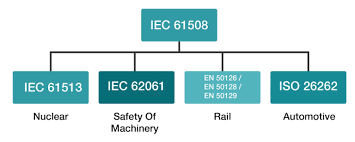
\includegraphics[width=1\textwidth]{Figuras/IEC61508.png}
        \centering\caption{Estándar IEC 61508.}
        \label{fig:IEC_61508}
    \end{figure}

    Dentro del universo de estándares ferroviarias, nos enfocaremos principalmente en tres de ellas: EN-50126 \cite{Paper_70,Paper_71,Paper_72,Paper_73,Paper_74}, EN-50128 \cite{Paper_75,Paper_74} y EN-50129 \cite{Paper_76,Paper_73}. Una falla en un sistema crítico puede poner en peligro cientos de vidas humanas y/o dañar la costosa infraestructura del sistema. Es por eso que los sistemas de enclavamiento deben cumplir los estrictos parámetros de fiabilidad, disponibilidad, mantenibilidad y seguridad (RAMS, del inglés Reliability, Availability, Mantenibility and Safety), durante todo el ciclo de vida definido en el estándar EN-50126 \cite{Paper_70,Paper_66,Paper_84}.

    Adicionalmente, el estándar EN-50126 define el nivel de integridad de seguridad (SIL, del inglés Safety Integrity Level). Este parámetro no es del sistema en su conjunto, sino que se asocia a las funciones de seguridad asociadas al sistema, pudiendo tener diferentes SILs dentro de un mismo dispositivo. Se definen cuatro niveles SIls, siendo el cuatro el nivel mas alto y, por lo tanto, el que tiene una tasa de fallas menor. Aunque existen diversos factores que impactan en la determinación del SIL, podemos tomar como referencia el criterio definido en la Tabla \ref{Tab:tabla_SIL} en función de la probabilidad de fallas por hora (PFH) del sistema funcionando de forma continua.

    \begin{table}[H]
        {
        \caption{SIL en función de la Probabilidad de Fallas/Hora (PFH).}
        \label{Tab:tabla_SIL}
        \centering
        %\small
            %\centering
            \begin{center}
            \resizebox{0.75\textwidth}{!}{
            \begin{tabular}{ c | c c c c c }
                %\hline	
                   SIL & & & & &  \\	
                \hline
                   4 & $10^{-8}$ & \multirow{4}{*}{$>$} & \multirow{4}{*}{PFH} & \multirow{4}{*}{$>$} & $10^{-9}$ \\
                   3 & $10^{-7}$ & &  & & $10^{-8}$ \\
                   2 & $10^{-6}$ & &  & & $10^{-7}$ \\
                   1 & $10^{-5}$ & &  & & $10^{-6}$ \\
                %\hline
            \end{tabular}
            }
            \end{center}
        }    
    \end{table}

    El estándar EN-50128 establece las buenas prácticas, metodologías y técnicas aplicables en el área de software para lograr el SIL objetivo. Algunas de estas técnicas pueden ser obligatorias, altamente recomendadas, recomendadas, desaconsejadas o prohibidas \cite{Paper_75,Paper_15,Paper_21,Paper_54,Paper_65}. En algunos casos es obligatorio elegir entre diferentes combinaciones de metodologías optativas. Podemos encontrar entre estas: evitar el uso de punteros, elegir un lenguaje fuertemente tipado, modularizar el código, prohibición de usar memoria dinámica, etc \cite{Paper_75}. Este estándar solo se aplica si el sistema incluye un microprocesador con software embebido.

    El estándar EN-50129 es el equivalente en hardware al estándar EN-50128. Las metodologías definidas en EN-50129 se centran en la elección de componentes electrónicos \cite{Paper_68,Paper_116,Paper_117,Paper_120,Paper_122,Paper_126}, compatibilidad electromagnética y dos conceptos fundamentales: redundancia \cite{Paper_23,Paper_29,Paper_32,Paper_42,Paper_49,Paper_97,Paper_98} y diversidad \cite{Paper_53,Paper_125,Paper_131,Paper_132,Paper_140,Paper_171}.

    
\subsection{Redundancia y diversidad en sistemas ferroviarios}

	La redundancia en sistemas críticos se define mediante la abreviatura NooM (N de M, del inglés, N out of M). Donde M representa la cantidad de módulos de medición/decisión que posee el sistema y N la cantidad de módulos que deben funcionar correctamente para que el sistema opere normalmente \cite{Paper_12,Paper_41,Paper_47,Paper_78,Paper_80,Paper_82,Paper_84}. En la Figura \ref{fig:redundancia} se puede apreciar un sistema con redundancia 2oo3, en el cual se tendrá una salida correcta siempre que se tenga a lo sumo un fallo por vez, no acumulativo. El sistema determina, mediante votación, la respuesta correcta a presentar como salida.
	
	\begin{figure}[H]
		\centering
		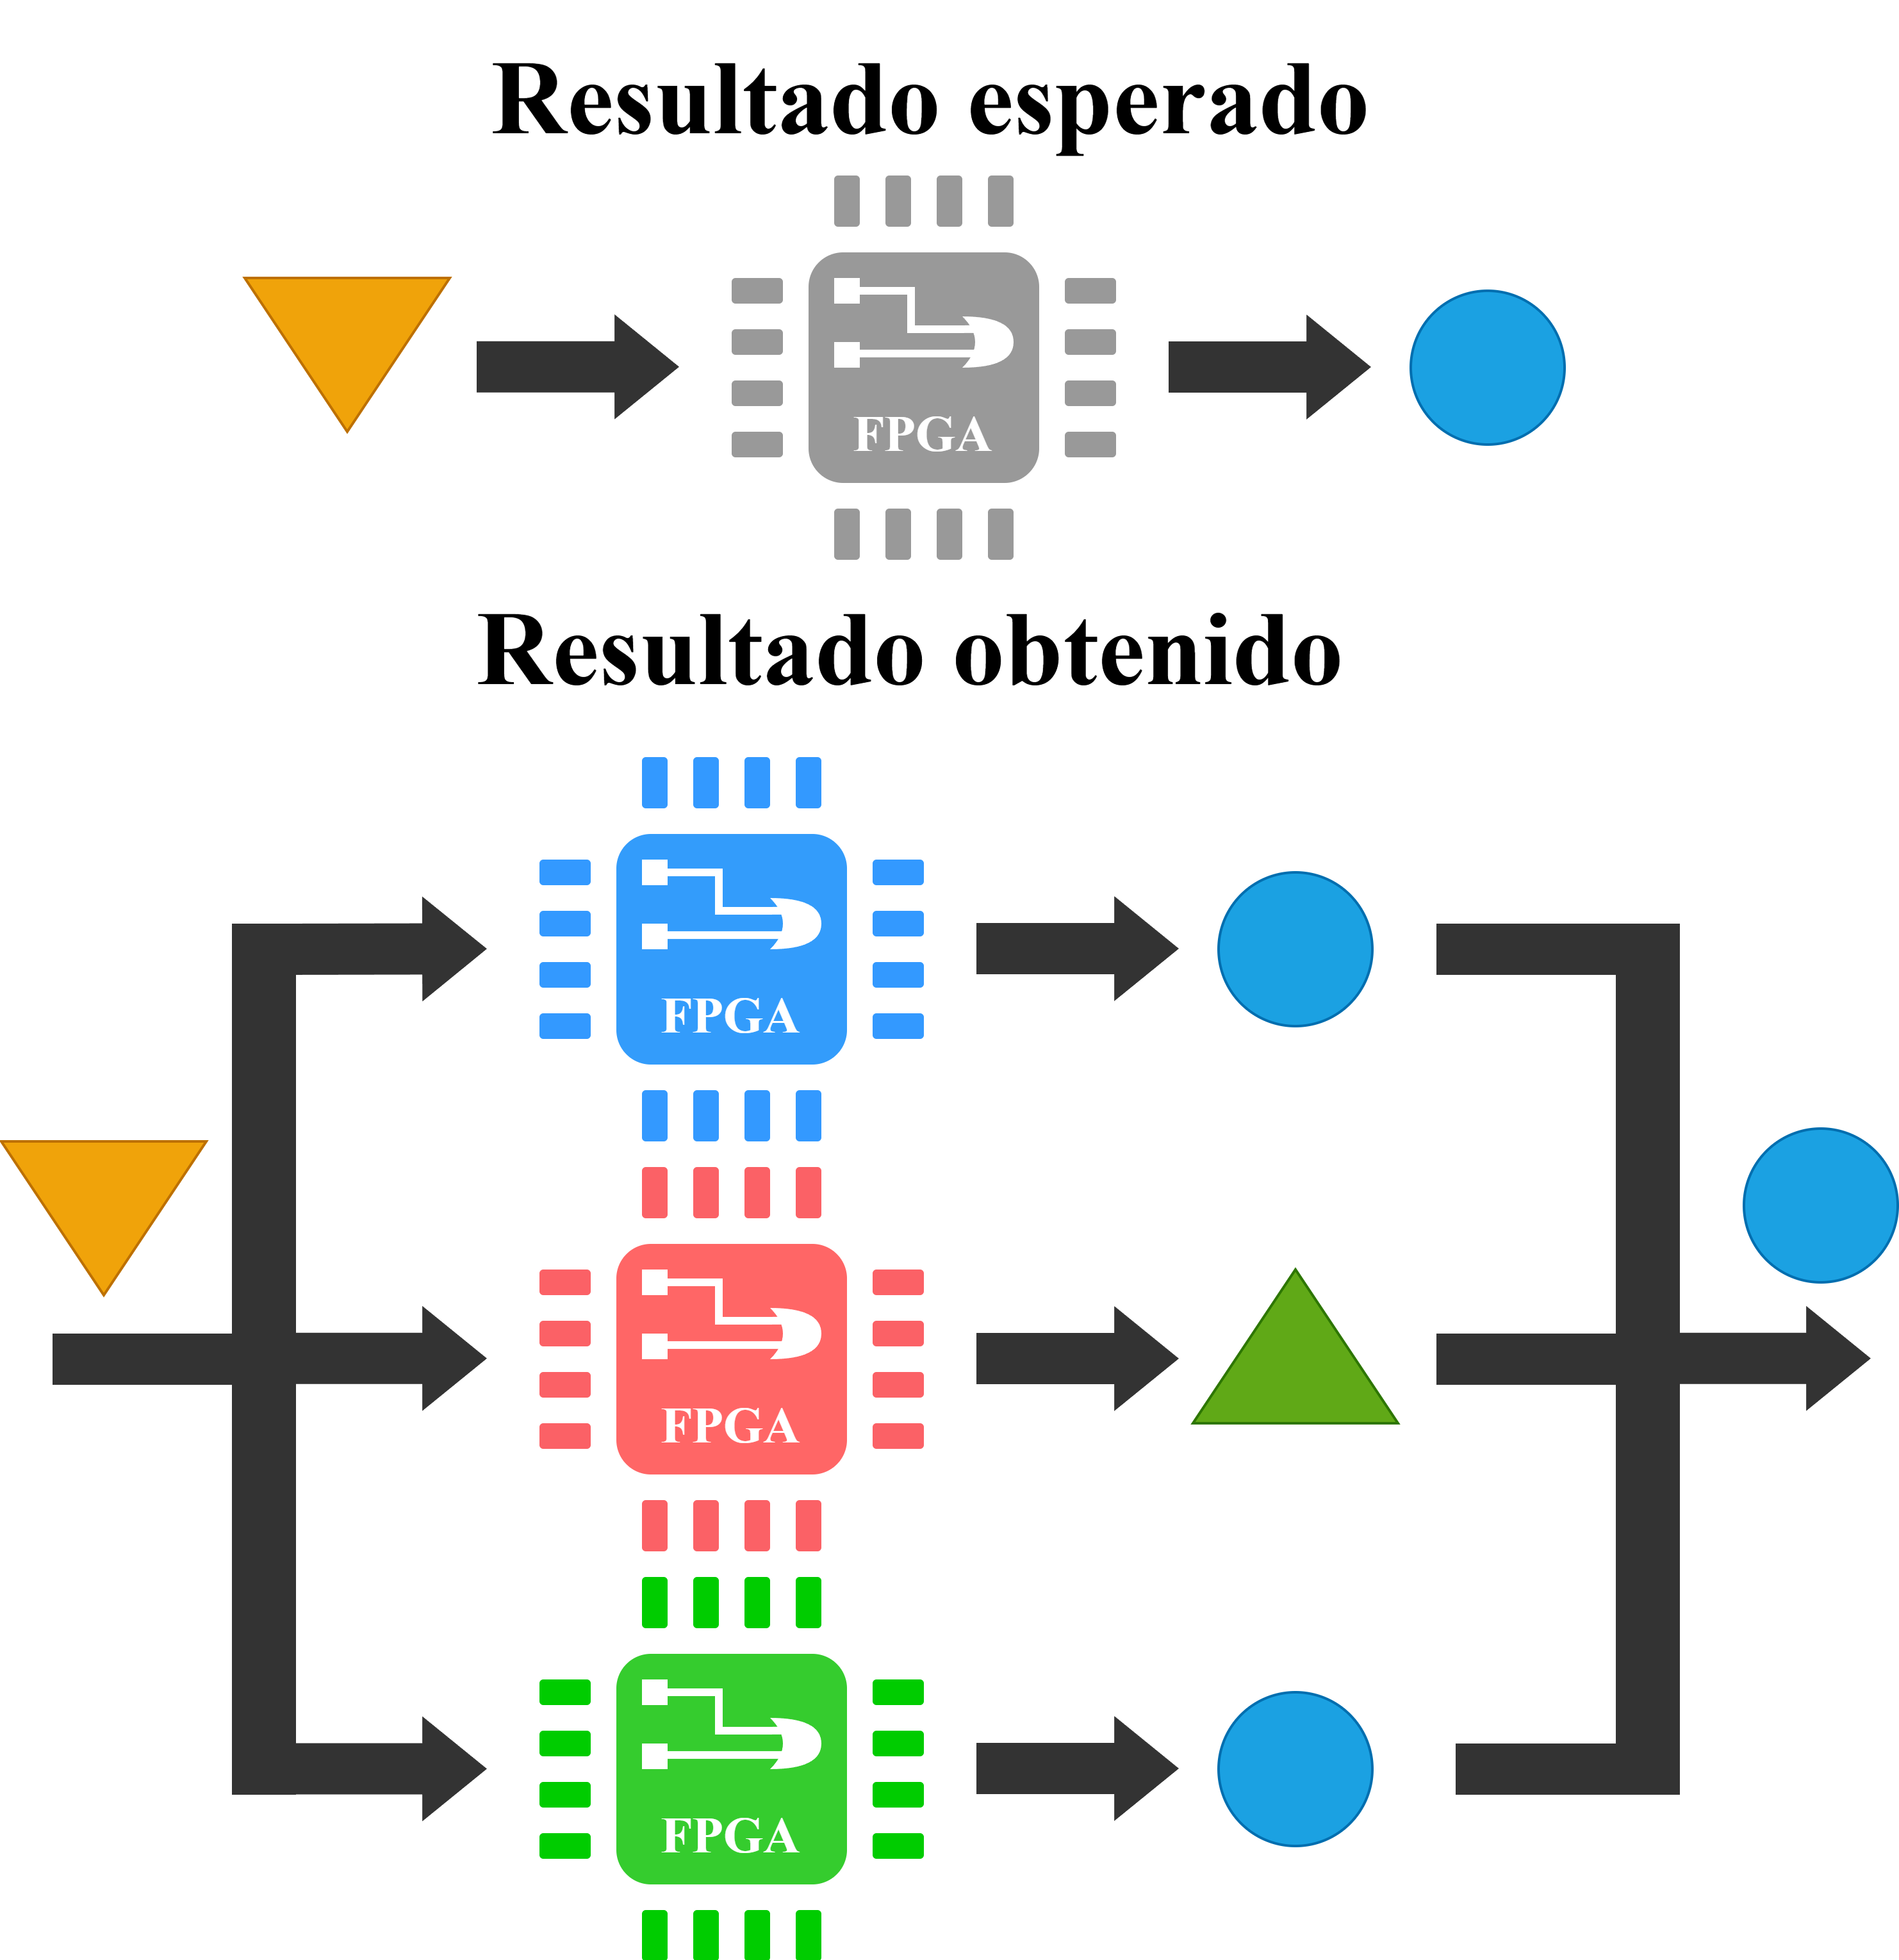
\includegraphics[width=1\textwidth]{Figuras/redundancia.png}
		\centering\caption{Sistema con redundancia 2oo3 y diversidad.}
		\label{fig:redundancia}
	\end{figure}
	
	La tasa de fallas de los sistemas utilizados debe ser lo mas pequeña posible. Existen fallas de causa común asociadas al fabricante de componentes, defectos eléctricos en los materiales, desperfectos en el software replicados en cada uno de los módulos, etc \cite{Paper_30,Paper_32,Paper_42,Paper_47,Paper_77,Paper_83,Paper_84,Paper_118,Paper_122,Paper_124,Paper_125,Paper_127,Paper_131,Paper_132,Paper_136,Paper_138,Paper_140}. Para mitigar las fallas de causa común y robustecer el sistema, se aplica el concepto de diversidad \cite{Paper_53,Paper_125,Paper_131,Paper_132,Paper_140,Paper_171}. En el caso de la Figura \ref{fig:redundancia}, esta diversidad está representada en los módulos de diferentes colores: azul, rojo y verde. De esta forma se busca simbolizar que los tres sistemas cumplen la misma función, pero de manera diferente (distintas plataforas y/o distinto lenguaje de programación o incluso diferente equipo de desarrollo). Los tres módulos tendrán, por lo tanto, tasas de falla distintas. Se asume, además, que los módulos pueden tener fallas simultáneas pero de probabilidad mucho mas baja que la tasa de fallas inherente a cada módulo.
	
	De la investigación realizada surge que el 66\% de las empresas utiliza una redundancia 2oo2 o 2oo3 para alcanzar los niveles de seguridad requeridos \cite{SIEMENS,ALSTOM,HITACHI,THALES,BOMBARDIER,KYOSAN,HIMA,CRRC,CAF,TRANSMASHHOLDING,HYUNDAI,GENERAL,CATERPILLAR,STADLER}. Solo una pequeña porción de las mismas utiliza redundancias 1oo2 \cite{ALSTOM} o 2oo4 \cite{HITACHI}. En consecuencia, se puede afirmar que una redundancia 2oo2 o 2oo3 es representativa de los sistemas analizados y puede utilizarse como esquema de partida para un diseño propio.
\section{RailTopoModel y RailML}
    \label{sec:railML}
    
    \subsection{RailTopoModel}

    En 2016 la UIC (del inglés, International Union of Railways) publicó el Standard 30100 \cite{Paper_109} en el cual definió un formato de intercambio de datos ferroviarios llamado RailTopoModel \cite{Paper_146,Paper_149,Paper_150,Paper_200}. RailTopoModel es un modelo topológico de infraestructura ferroviaria basado en grafos. El modelo abarca tres tipos de niveles, la topología de la red, objetos materiales, objetos inmateriales y objetos lógicos \cite{Paper_109}, tal como se ilustra en la Figura \ref{fig:RTM_3} (adaptada al español de \cite{Paper_109}). 

    \begin{figure}[H]
        \centering
        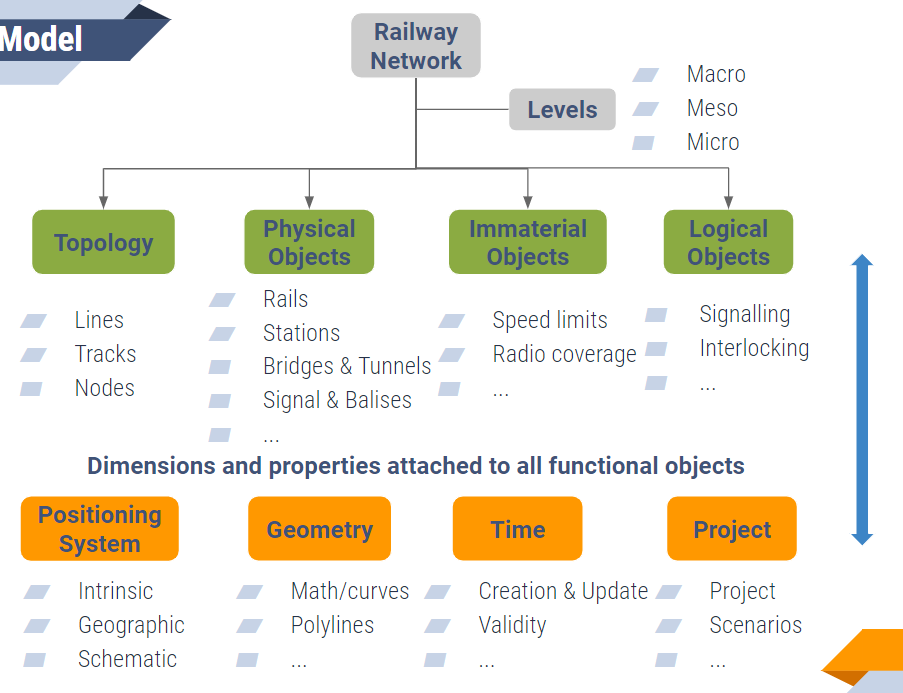
\includegraphics[width=1\textwidth]{Figuras/objetos}
        \centering\caption{Alcance del modelo de UIC RailTopoModel.}
        \label{fig:RTM_3}
    \end{figure}

    Cada uno de estos elementos posee propiedades y características propias, que pueden ser físicas o abstractas. Por ejemplo, los objetos materiales pueden ser adimensionales (señales, balizas, etc), unidimensionales (vías, plataformas, etc) o bidimensionales (estaciones, túneles, etc). Debido a cómo fue diseñado, RailTopoModel es un modelo muy apropiado para implementar un enfoque geográfico \cite{Paper_146,Paper_149,Paper_180,Paper_182,Paper_99,Paper_107}.
    
\subsubsection{Paquete base}

    El estándar RailTopoModel se divide en cuatro paquetes: la base, la topología, el posicionamiento y la red de entidades. La base incluye toda la información de alto nivel de la infraestructura que son comúnes a toda la red \cite{Paper_146}. Por ejemplo, el sistema de alimentación eléctrico utilizado puede ser por tercer riel o catenarias y este no cambia a lo largo de toda la red.

\subsubsection{Modelo de grafos}
    \label{sec:RTM}
    
    En el pasado, otros estudios han tratado de modelar el trazado ferroviario utilizando teoría de grafos \cite{Paper_9,Paper_101,Paper_102,Paper_103}. Pero todos ellos definían a las vías como las aristas del grafo y los cambios de vías como los nodos, lo cual dificultaba enormemente la inclusión de otros elementos ferroviarios como las plataformas, los pasos a nivel o los semáforos. RailTopoModel se apega mas a la teoría clásica de grafos y define como nodos a la unidad mínima de recursos físicos, llamándolos netElements y a la conexión física entre ellos como aristas, llamándolos netRelations \cite{Paper_109}.

    Un netElement debe contener un tramo de vía en su totalidad o varios tramos, pero un tramo de vía no puede tener varios netElements asociados. Opcionalmente, un netElement puede tener además cualquier otro elemento ferroviario asociado como plataformas, semáforos o balizas. Para entender mejor como se materializa este concepto se tiene la Figura \ref{fig:grafos_1} (adaptada al español de \cite{Paper_109}) que ejemplifica el modelado en grafos de una maquina de cambios.

    \begin{figure}[H]
        \centering
        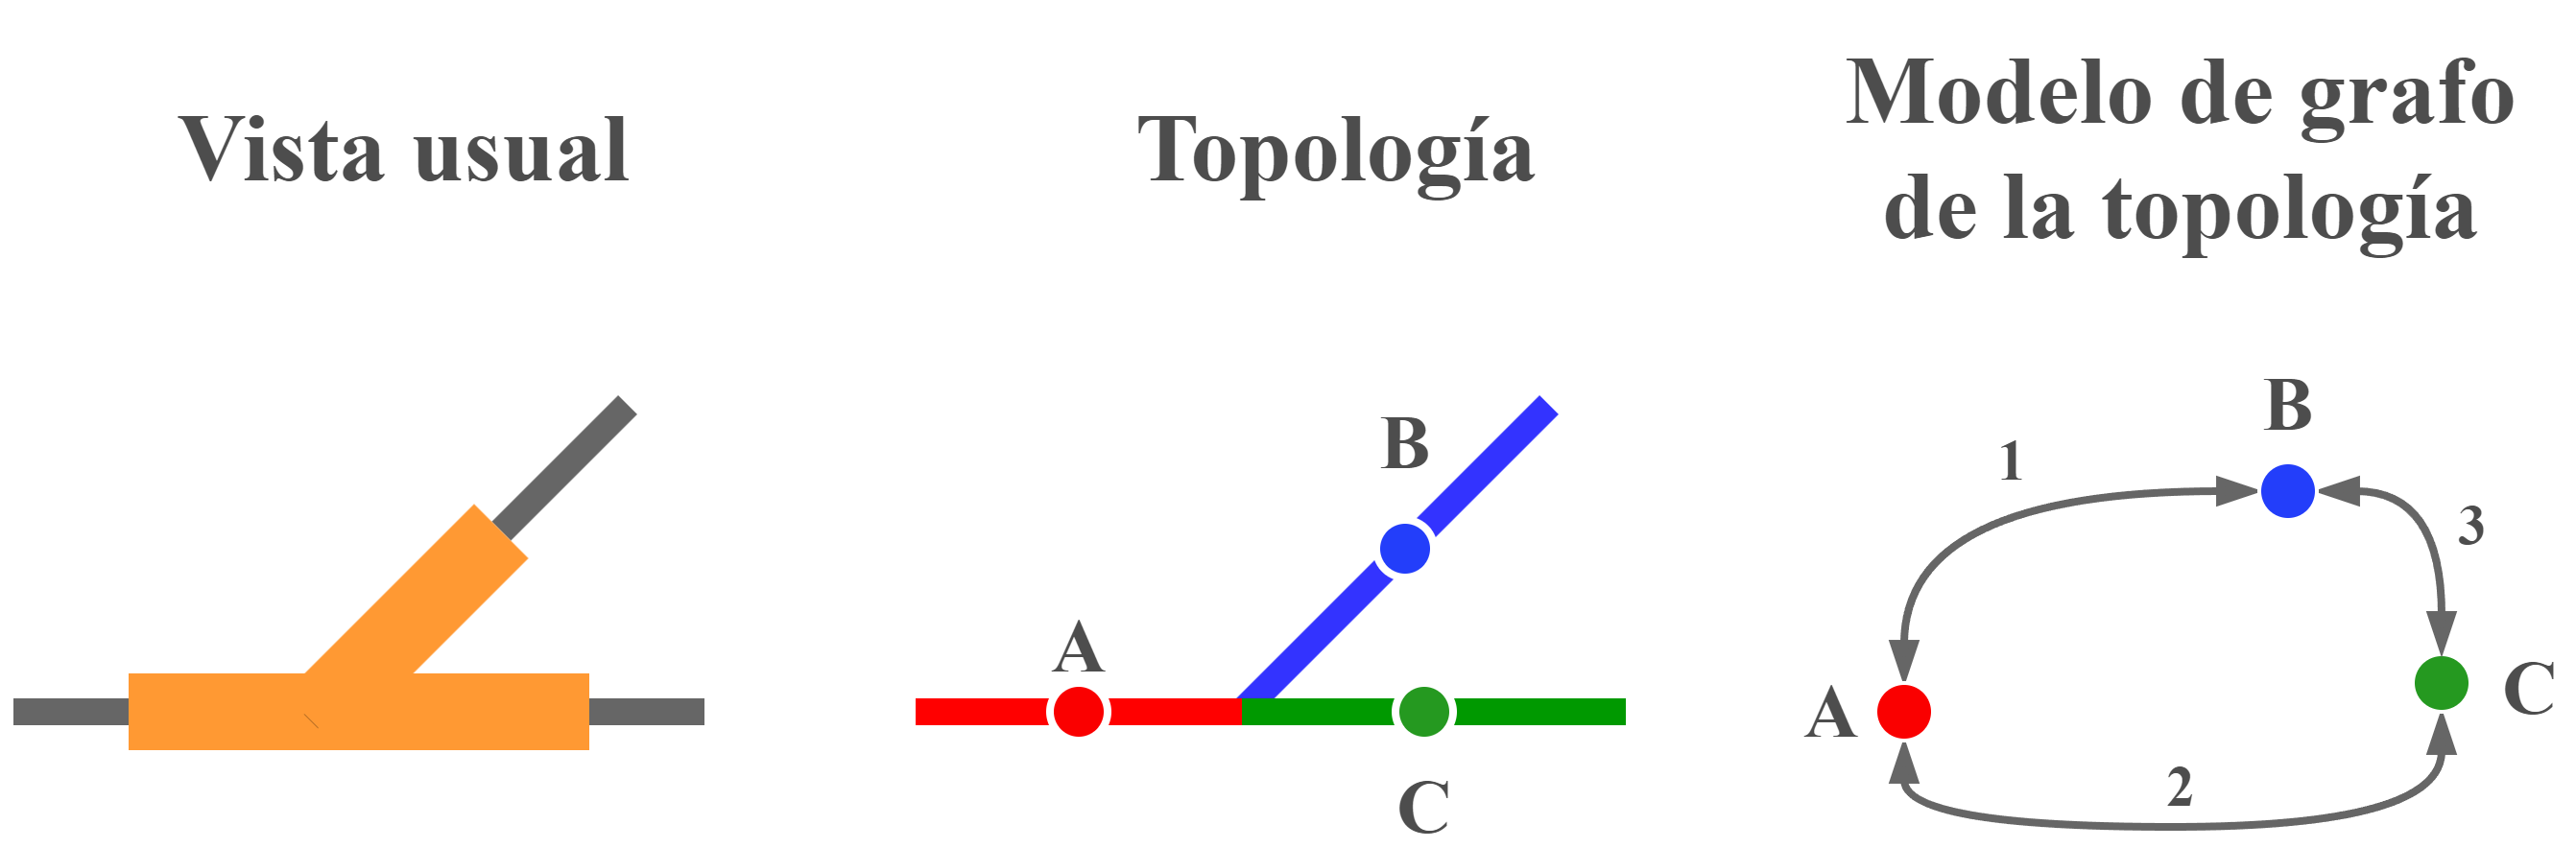
\includegraphics[width=1\textwidth]{Figuras/grafos}
        \centering\caption{Modelado en grafos de un cambio de vías simple.}
        \label{fig:grafos_1}
    \end{figure}

    En la Figura \ref{fig:grafos_1} se tiene un cambio de vías simple que conecta una vía de circulación (horizontal) con una vía de maniobras (oblicua). El netElement asociado a la vía principal antes de la bifurcación lo llamaremos A. Este netElement es también al que se asocia al objeto del cambio de vías simple. El netElement asociado a la vía de maniobras lo denominamos B y al asociado a la vía de continuación de la circulación lo denominamos C.

    En la representación del modelo de grafos, el netRelation 1 relaciona el netElement A y B de forma biyectiva. Es decir, A esta relacionado con B y B está relacionado con A. De la misma forma se asignan los netRelations 2 y 3. Sin embargo, no hay que confundir que dos vías estén conectadas con que un tren puede circular por ellas. Una formación podría circular por el tramo A-C, A-B, B-A y C-A, pero no podrá circular desde B hacia C sin pasar por A o viceversa. Es físicamente imposible que un tren realice ese movimiento de una sola maniobra. Para circular desde B hacia C primero deberá finalizar el tramo B-A, modificar la posición de la máquina de cambios y recorrer el tramo A-C. A la propiedad asignada a los netRelation que son físicamente transitables se la denomina navegabilidad y es una característica esencial de las redes de grafos que modelan redes ferroviarias. En este ejemplo, solo los netRelation 1 y 2 poseen navegabilidad. Los cambios de vías, sean estos simples, dobles o en tijeras, son los únicos elementos ferroviarios que alteran de forma dinámica la red ferroviaria y, por lo tanto, los únicos que afectan al parámetro de navegabilidad en los netElements adyacentes.
    
    
\subsubsection{Topología y niveles}

    La topología del modelo es una parte fundamental del estándar. RailTopoModel incluye el "principio de agregación", por el cual los elementos pueden ser agrupados en entidades mas grandes. En la Figura \ref{fig:RTM_1} se puede visualizar la estructura de capas propuesto por RailTopoModel (adaptada al español de \cite{Paper_109}).

    \begin{figure}[H]
        \centering
        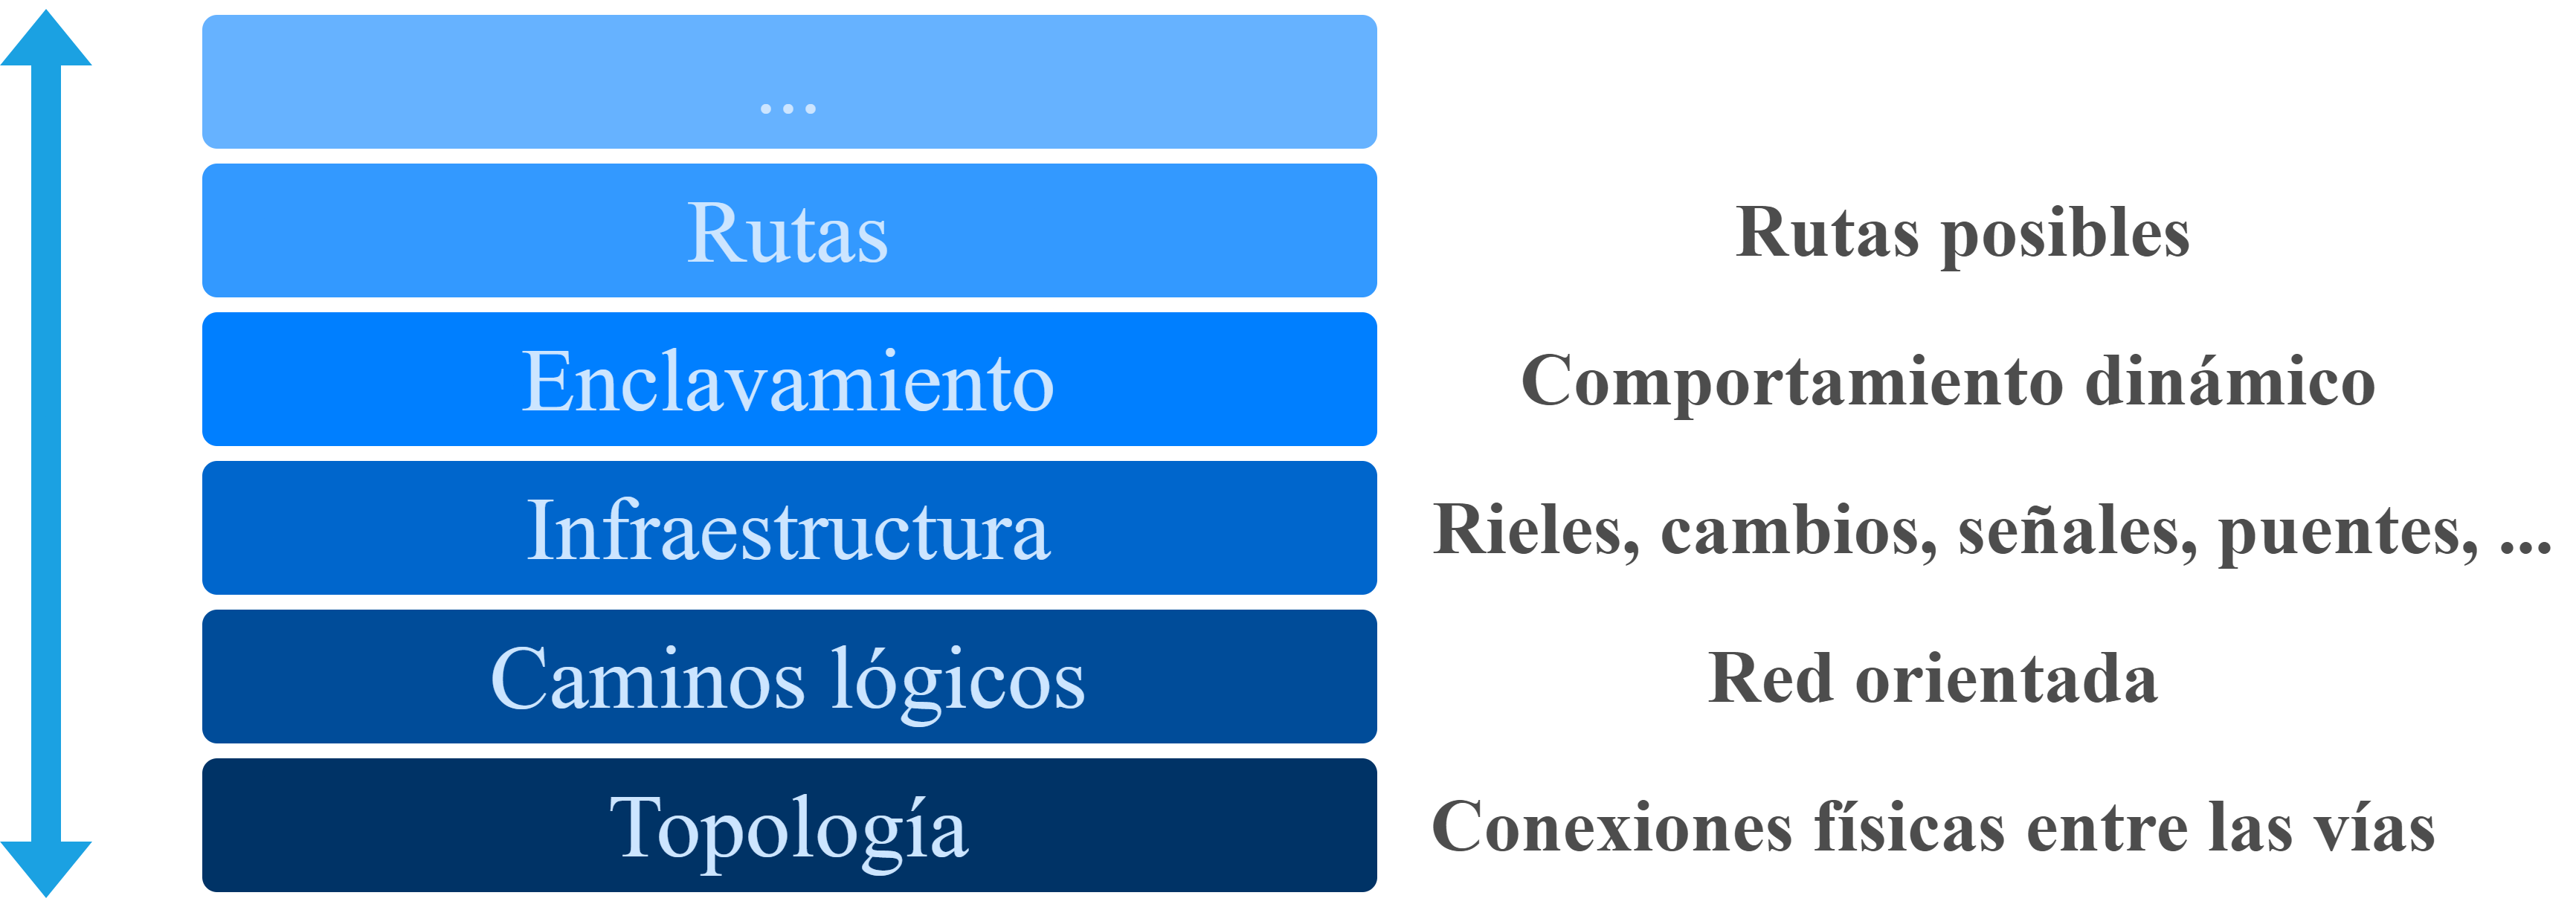
\includegraphics[width=1\textwidth]{Figuras/capas}
        \centering\caption{Estructura de capas de RailTopoModel.}
        \label{fig:RTM_1}
    \end{figure}
    
    La topología de la red está compuesta por los nodos (netElements) y las aristas (netRelations) que los conectan entre sí, lo cual constituye el nivel microscópico de la red. Cada nodo representa un tramo de vías que puede tener ciertos elementos ferroviarios asociados o ninguno. A su vez, los nodos pueden ser agrupados en diversos caminos lógicos, que son el conjunto de nodos cuyas relaciones y navegabilidad les permite constituir un camino físico entre ellos \cite{Paper_150}.

    A medida que se agrupan mas y mas cambios de vías junto con las plataformas y máquinas de cambios se constituye un punto de operación. La descripción en base a puntos de operación es a nivel mesoscópico, como se muestra en la Figura \ref{fig:RTM_2} (adaptada al español de \cite{Paper_109}), y es utilizado en logística. Las secciones de vía que no incluyen plataformas en las cuales las formaciones puedan detenerse se denominan secciones de líneas, o simplemente "líneas" dentro del modelo de RailTopoModel. La descripción que incluye tanto los puntos de operación como las secciones de líneas es a nivel macroscópico \cite{Paper_149}. Esta simplificación de la red es de gran importancia, ya que es ampliamente utilizada en los mapas ferroviarios de todas las estaciones del mundo: los puntos de operación son las estaciones y las secciones de línea son las vías que las comunican. 
    
    \begin{figure}[H]
        \centering
        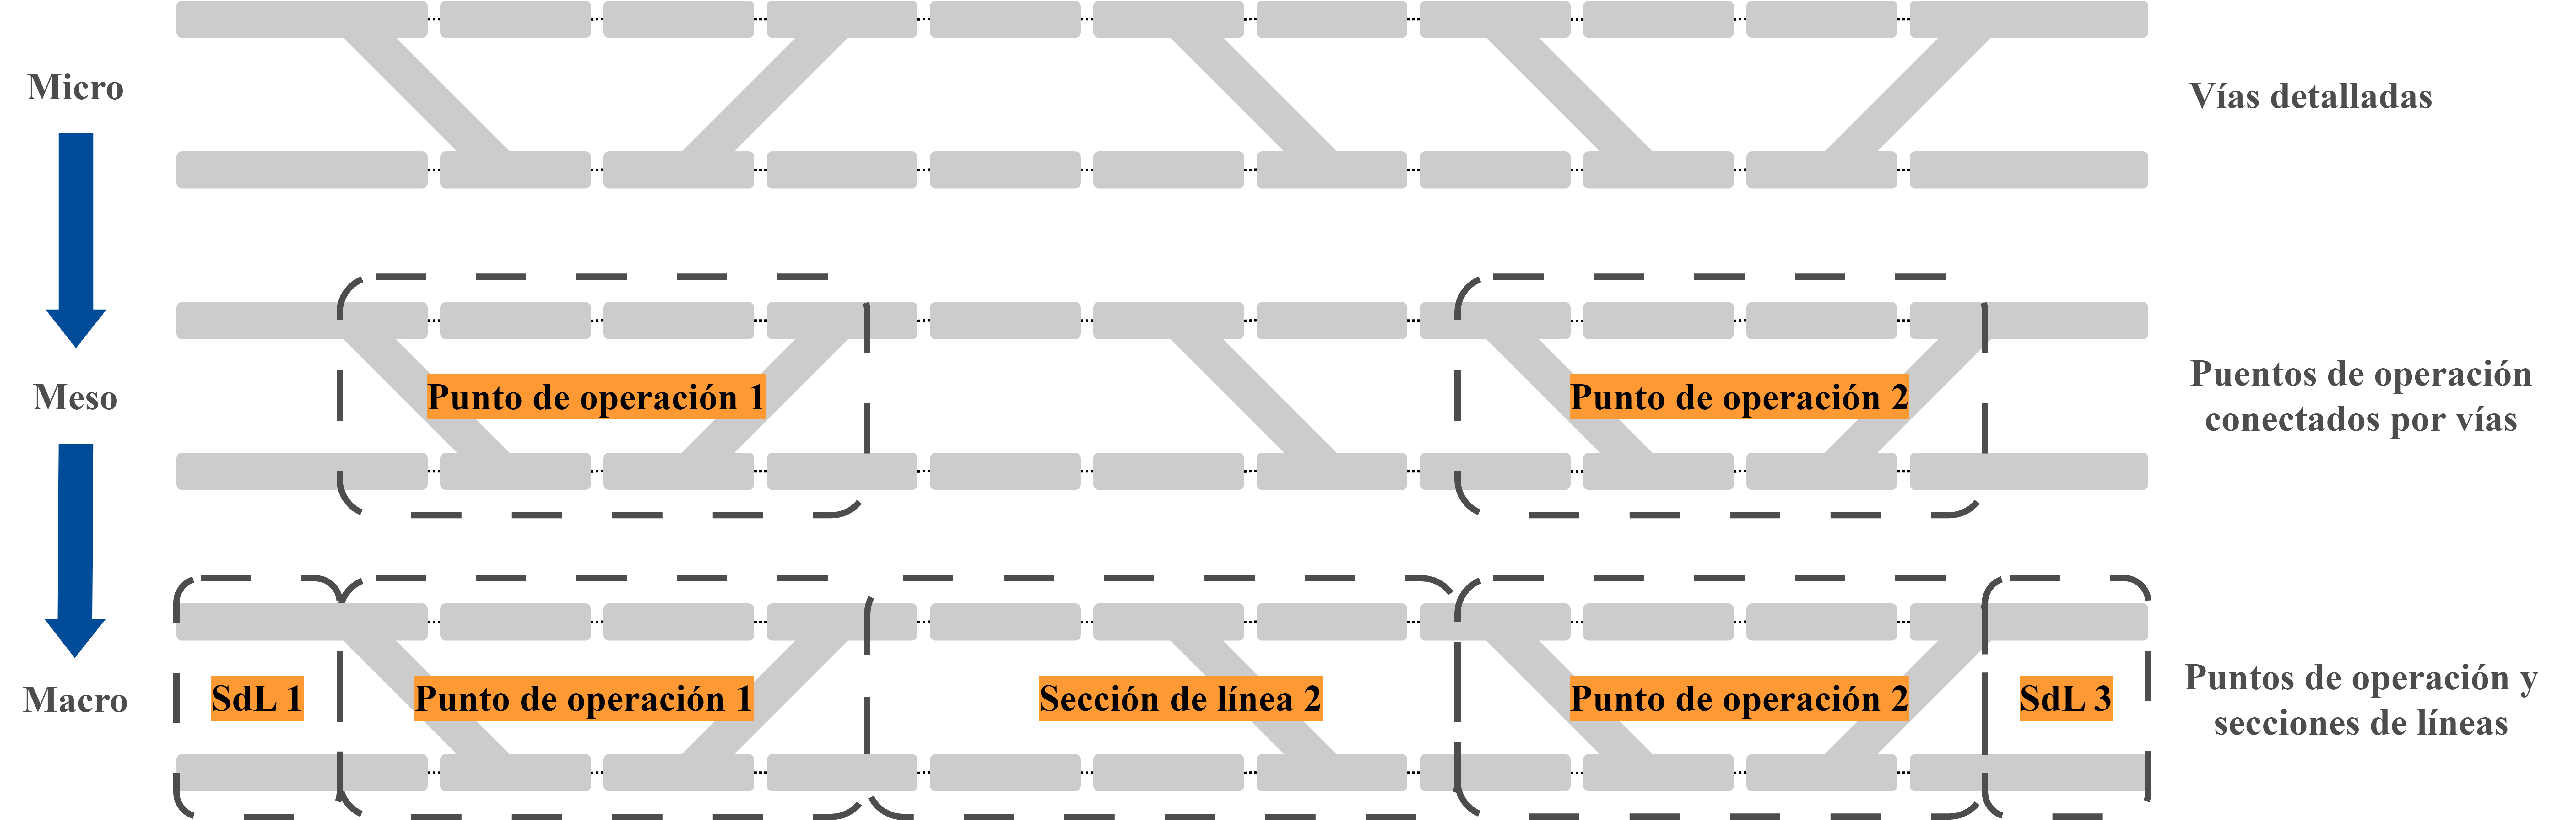
\includegraphics[width=1\textwidth]{Figuras/railtopomodel}
        \centering\caption{Niveles microscópico, mesoscópico y macroscópico.}
        \label{fig:RTM_2}
    \end{figure}
    
    Las instalaciones y sus propiedades constituyen todos los elementos ferroviarios asociados a un nodo. Estos representan elementos físicos del mundo real, pueden ser estáticos o dinámicos. Los elementos estáticos como los puentes, curvas y estaciones no alteran sus propiedades en ningún momento. Los elementos dinámicos como los pasos a nivel, máquinas de cambios o señales tienen algunas propiedades fijas, como la posición física del elemento, pero otras variables, como la posición mecánica de alguna de sus piezas o el estado eléctrico de sus circuitos \cite{Paper_146,Paper_150}.

    Un sistema de enclavamiento relaciona todos los módulos previamente mencionados. El sistema de enclavamientos modificará el estado de los elementos dinámicos, basados en el estado actual de los mismos, sometido a las restricciones impuestas por los elementos estáticos, buscando habilitar los caminos lógicos mas cortos y seguros entre un punto A y B.

    Finalmente, las rutas permitidas se obtienen a partir del estado de los elementos dinámicos decidido por el sistema y de definir el camino óptimo entre A y B que no comprometa la infraestructura del sistema. Todas las restricciones impuestas por las capas inferiores (caminos lógicos posibles, limitaciones de la infraestructura o estados previos que sean incompatibles con lo pedido) terminan emergiendo como un conjunto de rutas posibles de ser utilizadas, en detrimento de otras que, en ese instante de tiempo, no podrán ser habilitadas hasta que el estado del sistema se modifique.

    Como se puede apreciar, en este modelo, las rutas son una consecuencia de la infraestructura que se tiene y de los estados anteriores del sistema, producto de las rutas previamente pedidas. Un análisis completo de la topología e infraestructura permitiría obtener todo el conjunto de rutas posibles, para cualquier estado alcanzable por el sistema \cite{Paper_150}.
\subsubsection{Posicionamiento}

    RailTopoModel utiliza diferentes sistemas de posicionamiento: intrínseco, geográfico y esquemático \cite{Paper_112,Paper_150}. Las coordenadas intrínsecas se encuentran en el rango 0 a 1, relativas a la posición dentro del netElement. Estas coordenadas son obligatorias, junto con el largo asociado al netElement, independientemente de si se definieron o no las demás coordenadas. Las coordenadas geográficas son coordenadas absolutas, por ejemplo de un sistemas GPS. Finalmente las coordenadas esquemáticas son relativas a la posición del elemento dentro del archivo que modele ese sistema, muchas veces utilizadas en herramientas de software para posicionar los elementos en una interfaz gráfica.


    
    

	\subsection{RailML 3.0}

	railML \cite{RAILML_0,Paper_107,Paper_112,Paper_150,Paper_159} (del inglés, Railway Markup Language) es un estándar abierto de datos basado en XML, para intercomunicar aplicaciones ferroviarias. El estándar railML fue desarrollado por las principales empresas de la industria ferroviaria a partir del año 2001 \cite{Paper_159}. Las primeras dos versiones del estándar se diseñaron en base al enfoque funcional, pero en 2017 se lanzó railML 3.0 \cite{RAILML_0,Paper_146,Paper_150}, que adopta gran parte de los conceptos de RailTopoModel y los expande, al incorporar nuevos elementos que consideran las necesidades de las empresas ferroviarias que lo adoptan. Debido a la incorporación de RailTopoModel, railML 3.0 adopta un enfoque puramente geográfico \cite{Paper_150}.
	
	El estándar railML 3.0 posee cinco módulos principales:
	

    \begin{itemize}
        \item Common (CO) \cite{RAILML_CO}: similar al módulo base de RailTopoModel. Contiene datos transversales a todo el sistema, como el autor del archivo, el sistema eléctrico de alimentación, la versión de railML utilizada, etc.
        \item Infrastructure (IS) \cite{RAILML_IS}: incorpora al módulo de topología de RailTopoModel, con sus netElement y netRelations. Además, incorpora el sistema de coordenadas, la geometría y todos los elementos ferroviarios. En estos últimos solo admite datos estáticos como la posición, tamaño y demás atributos invariantes en el tiempo.
        \item Interlocking (IL) \cite{RAILML_IL}: incorpora los atributos dinámicos de los elementos ferroviarios mencionados en la infraestructura y agrega el listado de rutas.
        \item Rollingstock (RS) \cite{RAILML_RS}: incorpora toda la información relativa al material rodante: coches, vagones, locomotoras, formaciones combinadas, etc.
        \item Timetable and Rostering (TT) \cite{RAILML_TT}: incorpora detalles logísticos de la red ferroviaria.
    \end{itemize}

    A lo largo de esta tesis doctoral nos enfocaremos exclusivamente en los tres primeros módulos. Los cuales serán analizados detalladamente a medida que sea necesario introducirlos.
	\subsection{Uso del estándar railML en la industria ferroviaria}

    El estándar railML es promovido por empresas de gran peso en la industria ferroviaria como Siemens, Thales, Alstom, CAF, ADIF y Toshiba, que concentrán la mayoría de la cuota de mercado global \cite{PARTNERS}. Adicionalmente, diversas instituciones y organismos ferroviarios a nivel estatal y nacional hacen uso del estándar railML en sus desarrollos ferroviarios \cite{PARTNERS}, tales como: Queensland Rail, Transdev Deutschland, Transperth, Saudi Railway Company y Transport for New South Wales, entre otras.

    En sus primeros años de vida railML experimentó varios cambios, pero no fue hasta su versión 3.0 con enfoque geográfico que el uso del estándar creció exponencialmente. Entre el 40 y el 60\% de sus usuarios adoptaron el estándar en los últimos siete años \cite{PARTNERS}.

    Podemos encontrar las herramientas mas diversas basadas en railML: analizadores de infraestructura \cite{MAPREX}, planificador logístico para material rodante \cite{IVU}, visualizadores de datos \cite{RAILVIVID}, planificadores de infraestructura \cite{VISALL3D} y visualizadores/simuladores de infraestructura enclavamiento \cite{DESIGN4RAIL}. Muchas de ellas certificadas e intercompatibles entre sí. Aunque la mayoría son herramientas de código cerrado, el estándar railML es abierto y sigue un principio bottom-top: todas las necesidades de la industria son tenidas en cuenta para ser incorporadas en nuevas versiones del estándar, siguiendo el exitoso modelo del estándar USB, Bluetooth y GSM. 
\section{Estado del arte}

\lipsum[1]

\subsection{Empresas del sector ferroviario}

\lipsum[1]
\subsection{Herramientas existentes}

\lipsum[1]
\subsection{Estudios realizados}

\lipsum[1]
\subsection{Enfoque funcional vs enfoque geografico}

\lipsum[1]

\subsection{RailTopoModel}

\lipsum[1]

\subsubsection{Modelo de grafos}

\lipsum[1]
\subsubsection{Topología y niveles}

    La topología del modelo es una parte fundamental del estándar. RailTopoModel incluye el "principio de agregación", por el cual los elementos pueden ser agrupados en entidades mas grandes. En la Figura \ref{fig:RTM_1} se puede visualizar la estructura de capas propuesto por RailTopoModel.

    \begin{figure}[!h]
        \centering
        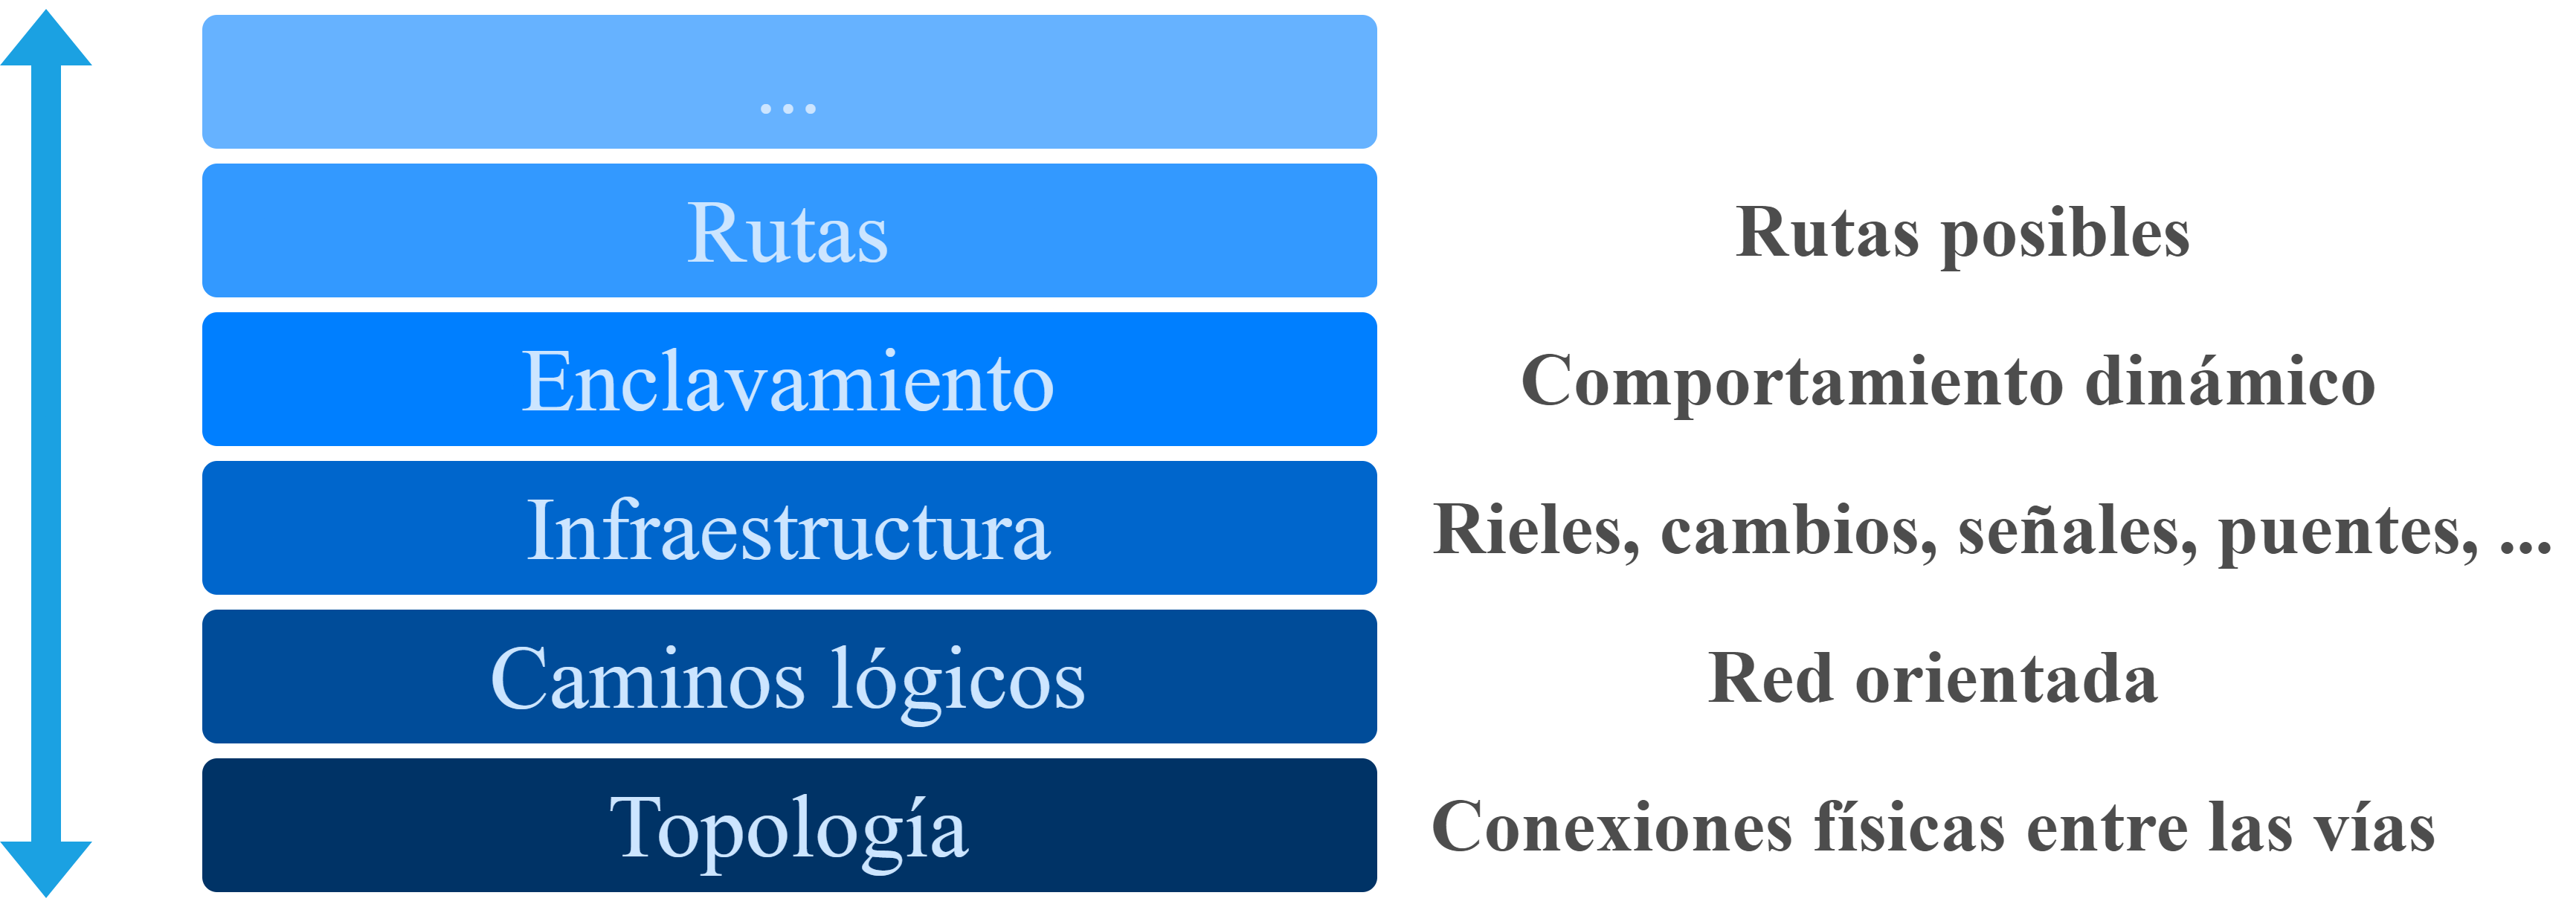
\includegraphics[width=1\textwidth]{Figuras/capas}
        \centering\caption{Estructura de capas de RailTopoModel.}
        \label{fig:RTM_1}
    \end{figure}
    
    La topología de la red está compuesta por los nodos (netElements) y las aristas (netRelations) que los conectan entre sí, lo cual constituye el nivel microscópico de la red. Cada nodo representa un tramo de vías que puede tener ciertos elementos ferroviarios asociados o ninguno. A su vez, los nodos pueden ser agrupados en diversos caminos lógicos, que son el conjunto de nodos cuyas relaciones y navegabilidad les permite constituir un camino físico entre ellos.

    A medida que se agrupan mas y mas cambios de vías junto con las plataformas y máquinas de cambios se constituye un punto de operación. La descripción en base a puntos de operación es a nivel mesoscópico, como se muestra en la Figura \ref{fig:RMT_2}, y es utilizado en logística. Las secciones de vía que no incluyen plataformas en las cuales las formaciones puedan detenerse se denominan secciones de líneas, o simplemente "líneas" dentro del modelo de RailTopoModel. La descripción que incluye tanto los puntos de operación como las secciones de líneas es a nivel macroscópico. Esta simplificación de la red es de gran importancia, ya que es ampliamente utilizada en los mapas ferroviarios de todas las estaciones del mundo: los puntos de operación son las estaciones y las secciones de línea son las vías que las comunican. 
    
    \begin{figure}[!h]
        \centering
        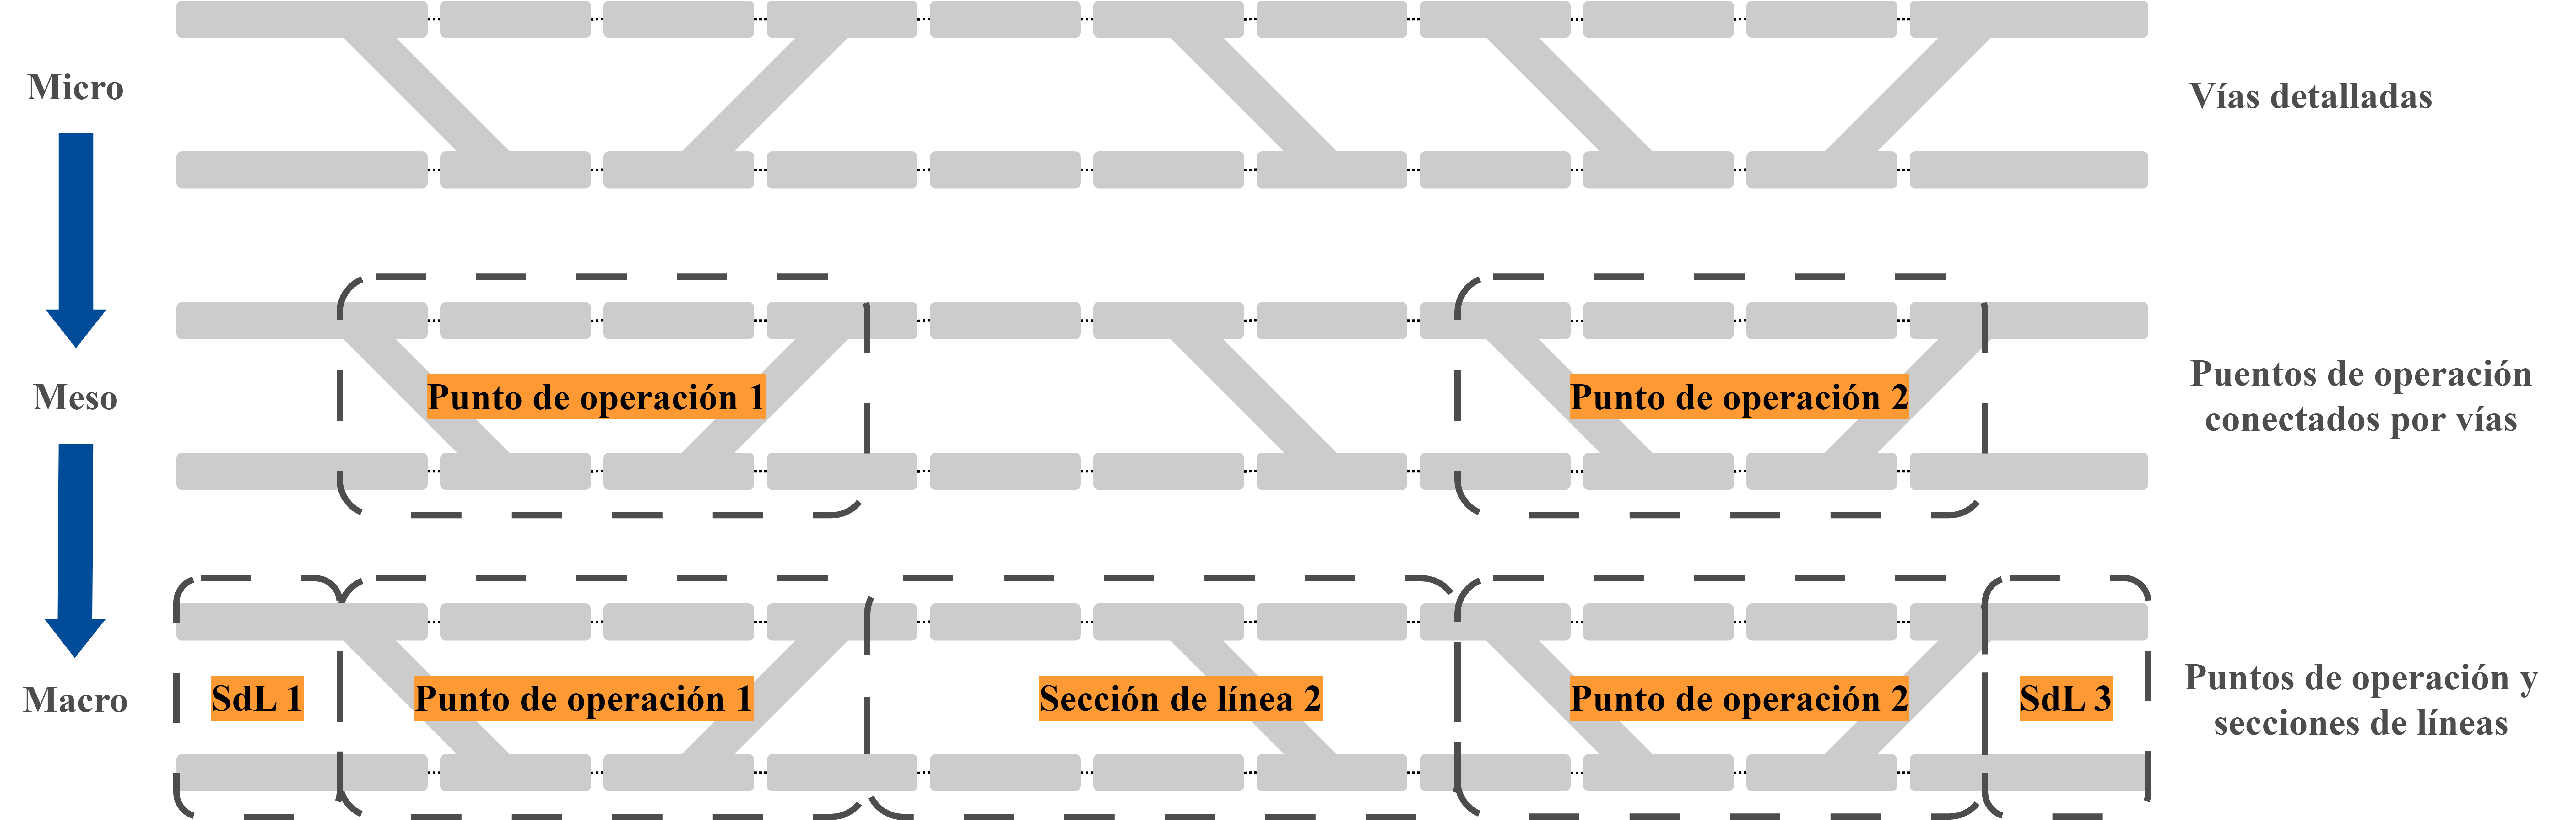
\includegraphics[width=1\textwidth]{Figuras/railtopomodel}
        \centering\caption{Niveles microscópico, mesoscópico y macroscópico.}
        \label{fig:RTM_2}
    \end{figure}
    
    Las instalaciones y sus propiedades constituyen todos los elementos ferroviarios asociados a un nodo. Estos representan elementos físicos del mundo real, pueden ser estáticos o dinámicos. Los elementos estáticos como los puentes, curvas y estaciones no alteran sus propiedades en ningún momento. Los elementos dinámicos como los pasos a nivel, máquinas de cambios o señales tienen algunas propiedades fijas, como la posición física del elemento, pero otras variables, como la posición mecánica de alguna de sus piezas o el estado eléctrico de sus circuitos.

    Un sistema de enclavamiento relaciona todos los módulos previamente mencionados. El sistema de enclavamientos modificará el estado de los elementos dinámicos, basados en el estado actual de los mismos, sometido a las restricciones impuestas por los elementos estáticos, buscando habilitar los caminos lógicos mas cortos y seguros entre un punto A y B.

    Finalmente, en base al estado de los elementos dinámicos decidido por el sistema de enclavamiento, buscando el camino óptimo entre A y B que no comprometa la infraestructura del sistema, es que obtenemos las rutas permitidas. Todas las restricciones impuestas por las capas inferiores (caminos lógicos posibles, limitaciones de la infraestructura o estados previos que sean incompatibles con lo pedido) terminan emergiendo como un conjunto de rutas posibles de ser utilizadas, en detrimento de otras que, en ese instante de tiempo, no podrán ser habilitadas hasta que el estado del sistema se modifique.

    Como se puede apreciar, en este modelo, las rutas son una consecuencia de la infraestructura que se tiene y de los estados anteriores del sistema, producto de las rutas previamente pedidas. Un análisis completo de la topología e infraestructura permitiría obtener todo el conjunto de rutas posibles, para cualquier estado alcanzable por el sistema.
\subsection{RailML}
    \label{sec:railML}
    
    railML [REF] (del inglés, Railway Markup Language) es un estándar abierto de comunicación de datos entre herramientas ferroviarias desarrollado por las principales empresas de la industria ferroviaria a partir del año 2002. Las primeras dos versiones del estándar se diseñaron en base al enfoque funcional, pero en 2017 se lanzó railML 3.0, basado en RailTopoModel y, por lo tanto, adoptando un enfoque puramente geográfico.

\subsubsection{RailML 3.0}

\lipsum[1]
\subsubsection{Uso del estándar railML en la industria ferroviaria}

    El estándar railML es promovido por empresas de gran peso en la industria ferroviaria como Siemens, Thales, Alstom, CAF, ADIF y Toshiba, que concentrán la mayoría de la cuota de mercado global [REF]. Adicionalmente, diversas instituciones y organismos ferroviarios a nivel estatal y nacional hacen uso del estándar railML en sus desarrollos ferroviarios [REF], tales como: Queensland Rail, Transdev Deutschland, Transperth, Saudi Railway Company y Transport for New South Wales, entre otras.

    En sus primeros años de vida railML experimentó varios cambios, pero no fue hasta su versión 3.0 con enfoque geográfico que el uso del estándar creció exponencialmente. Entre el 40 y el 60\% de sus usuarios adoptaron el estándar en los últimos siete años [REF].

    Podemos encontrar las herramientas mas diversas basadas en railML: analizadores de infraestructura [MAPREX], planificador logístico para material rodante [IVU], visualizadores de datos [railViVid], planificadores de infraestructura [VIS ALL 3D] y visualizadores/simuladores de infraestructura enclavamiento [D4R]. Muchas de ellas certificadas e intercompatibles entre sí. Aunque la mayoría son herramientas de código cerrado, el estándar railML es abierto y sigue un principio bottom-top: todas las necesidades de la industria son tenidas en cuenta para ser incorporadas en nuevas versiones del estándar, siguiendo el exitoso modelo del estándar USB, Bluetooth y GSM. 
\section{Herramienta propuesta}

    El objetivo de esta tesis es el desarrollo de una herramienta que realice automáticamente tanto el diseño del señalamiento como la implementación del sistema de enclavamiento en una plataforma electrónica y la generación de una interfaz gráfica a medida de cada locación ferroviaria. El flujo de trabajo mostrado en la Figura \ref{fig:workflow} introduce el Analizador de Redes Ferroviarias (RNA, del inglés, Railway Network Analyzer), el Generador Automático de Código (ACG, del inglés, Automatic Code Generator) y el Generador Automático de Interfaz Gráfica (AGG, del inglés, Automatic Graphic User Interface Generator). Cada flecha indica las relaciones entre los diferentes bloques. El RNA se enfoca principalmente en el comportamiento estático del sistema, mientras que el ACG se enfoca en el comportamiento dinámico. El AGG se enfoca en generar una interfaz gráfica acorde al señalamiento generado por el ACG y en establecer la comunicación entre la interfaz gráfica y la plataforma FPGA. Cada una de estas herramientas desarrolladas se explican en profundidad en esta memoria: RNA en el Capítulo \ref{sec:RNA}, ACG en el Capítulo \ref{sec:ACG} y AGG en el Capítulo \ref{sec:AGG}.

    \begin{figure}[H]
        \centering
        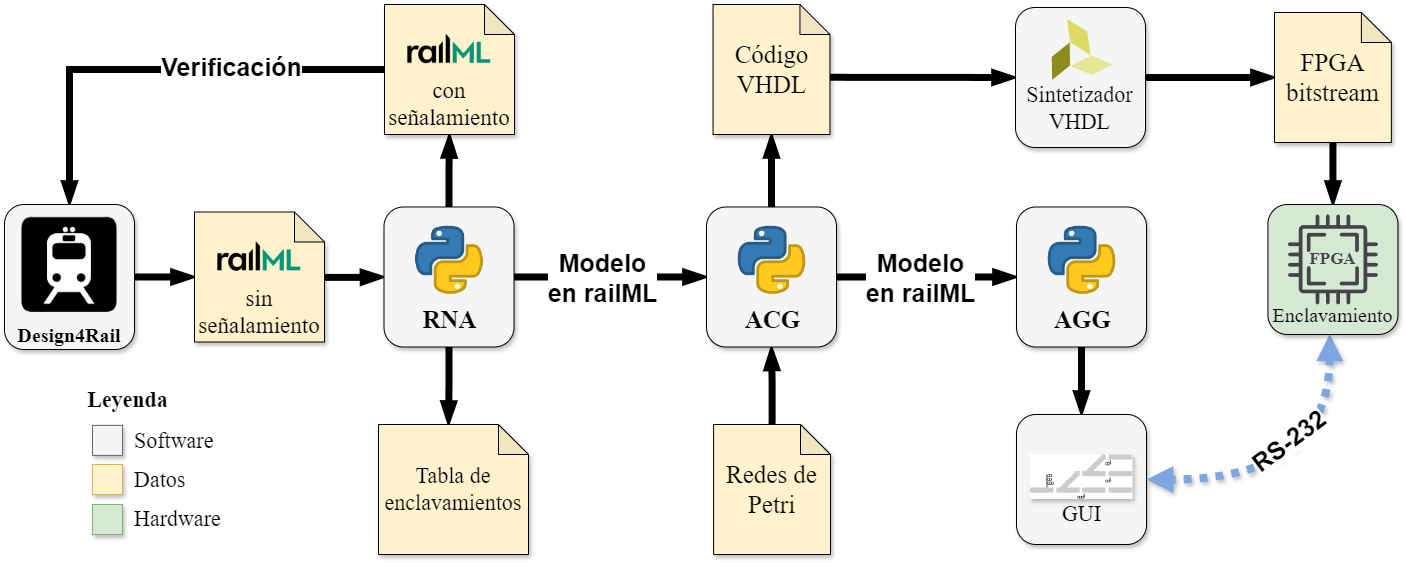
\includegraphics[width=1\textwidth]{Figuras/workflow.png}
        \centering\caption{Flujo de trabajo de la presente tesis.}
        \label{fig:workflow}
    \end{figure}

    El RNA importa un archivo en formato railML que describe el sistema, con o sin señalamiento previo. Luego el RNA analiza la topología de la red, detecta todos los elementos ferroviarios involucrados y genera el señalamiento necesario para que la red sea segura. Finalmente, el RNA exporta un nuevo archivo en formato railML con el nuevo señalamiento, además de la tabla de enclavamientos del sistema, con todas las rutas soportadas por esa red ferroviaria. El nuevo archivo railML es utilizado por el ACG para generar código en VHDL \cite{Paper_206} (del inglés, Very High-Speed Integrated Circuit Hardware Description Language) automáticamente para ser sintetizado en una plataforma FPGA \cite{Paper_8,Paper_25,Paper_34,Paper_46,Paper_49} (del inglés, Field Programmable Gate Arrays). A su vez, el modelo en railML generado por el RNA, junto con información referida al código generado, es utilizado por el AGG para generar una interfaz gráfica a medida de la locación ferroviaria, junto con el manejo de la comunicación entre la interfaz y la plataforma electrónica utilizada.
    
    El proceso de validación, que se realiza para saber si las herramientas desarrolladas funcionan correctamente, incluye la validación de la sintaxis del archivo railML generado por el RNA, la validación de la tabla de enclavamiento generada automáticamente por el RNA y, finalmente, la validación del señalamiento generado conforme a los principios de señalamiento (Sección \ref{sec:principios}). Para implementar automáticamente un sistema de enclavamiento, el ACG toma este diseño de señalamiento estático generado automáticamente y un modelo de comportamiento dinámico en redes de Petri, diseñado por el autor de esta tesis de doctorado. 

\subsection{Enfoque aplicado}

    Durante la Maestría en Sistemas Embebidos se desarrollo un primer prototipo del ACG en base a un rudimentario modelo de redes de grafos \cite{Paper_206}. Fue este modelo de grafos el que permitió probar el ACG con una amplia variedad de topologías, debido a la flexibilidad, linealidad y escalabilidad del modelo \cite{Paper_109,Paper_149,Paper_150}. En esta etapa temprana del proyecto ya se había adoptado un enfoque geográfico.

    La única desventaja de la elección temprana de un enfoque geográfico fue la, aparente, inexistencia de herramientas o soportes formales, para lo cual era necesario desarrollar todo desde cero sin un estándar que lo sostenga. Aún así, una vez desarrollada la herramienta se podía reutilizar innumerables veces, por lo que las ventajas a largo plazo eran mayores que realizar un diseño a mano, a medida de cada locación. Al descubrir la existencia de railML, rápidamente se comenzó la migración del ACG para ser compatible con el estándar.

    El desarrollo del RNA fue posterior al desarrollo del ACG, y fue completamente en línea con el estándar railML desde un inicio. Al ser compatibles con railML, tanto el RNA como el ACG deben ser compatibles también con el modelo planteado por RailTopomodel. Debido a esto, el desarrollo de la herramienta siguió indefectiblemente los lineamientos de un enfoque geográfico.
    
    El AGG se desarrolló en las etapas finales del doctorado, aprovechando el enfoque geográfico y el gran nivel de detalle que obtiene el RNA de cada archivo railML. El objetivo fue obtener una interfaz que simplificase tanto la transmisión de los comandos, cómo la recepción y la representación de los estados del señalamiento y el enclavamiento.
\subsection{Arquitectura del sistema}

	En el flujo de trabajo de la presente tesis, ilustrado en la Figura \ref{fig:workflow}, se destacan las tres herramientas interconectadas como parte central de la solución propuesta: el RNA, el ACG y el AGG. Como se ilustra en la Figura \ref{fig:architecture}, existen diferentes módulos a considerar en cada una de las tres herramientas. Los módulos en amarillo corresponden a las clases implementadas en base al estándar railML, los módulos en verde son aquellos algoritmos originales necesarios para resolver el problema, y finalmente los módulos en violeta constituyen todas las validaciones realizadas. 

    \begin{figure}[H]
        \centering
        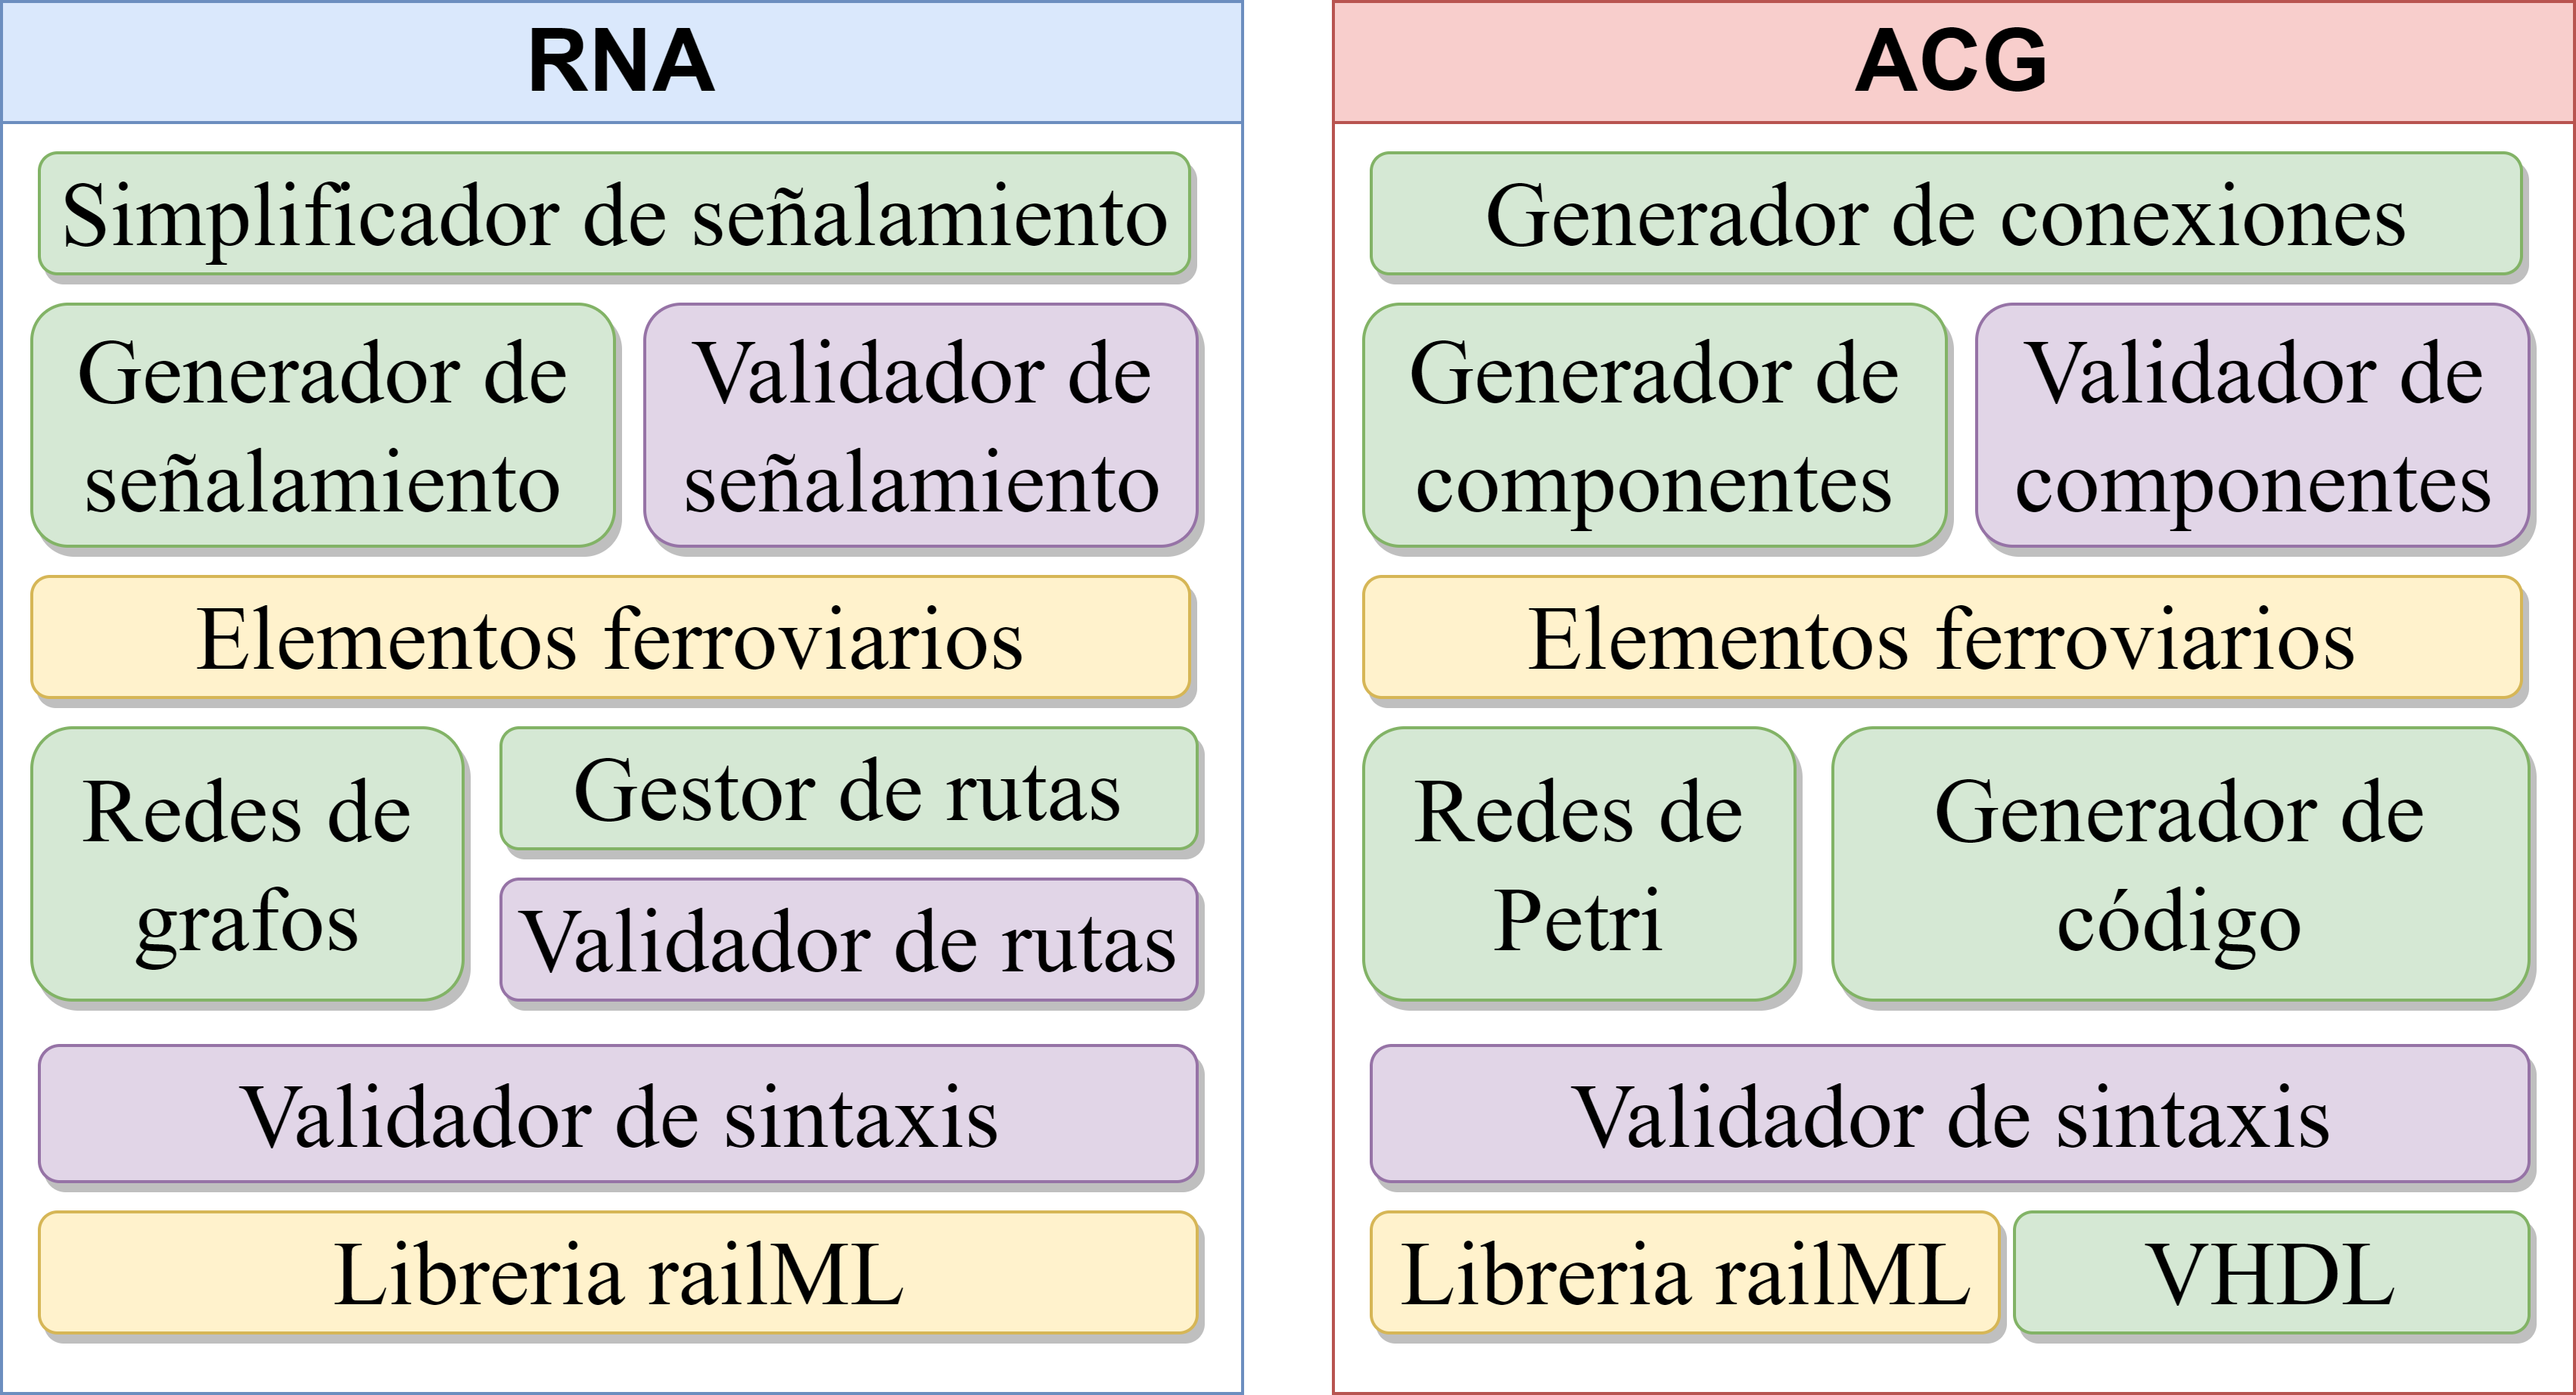
\includegraphics[width=1\textwidth]{Figuras/Architecture.png}
        \centering\caption{Arquitectura del sistema}
        \label{fig:architecture}
    \end{figure}

    Las clases implementadas se corresponden una a una con las definidas en el estándar railML. De esta manera, cualquier elemento definido en un archivo railML tendrá su equivalente en el modelo de datos utilizado. La biblioteca a implementar debe ser capaz de importar, modificar y exportar archivos en formato railML. Además, la librería debe contemplar todos los atributos que railML defina para cada elemento ferroviario.

    Respecto al RNA, el análisis de redes de grafos es explicado en la Sección \ref{sec:grafos}, la generación de señalamiento en la Sección \ref{sec:generacion}, la simplificación del señalamiento en la Sección \ref{sec:simplificacion} y, finalmente, la generación de rutas ferroviarias y la tabla de enclavamientos es explicado en la Sección \ref{sec:rutas}. En tanto que para el ACG, la descripción de cada bloque implementado se encuentra explicada en la Sección \ref{sec:interlockingArch}, la implementación de la redundancia en la Sección \ref{sec:network} y la plataforma utilizada se explica en la Sección \ref{sec:plataforma}. Finalmente, el AGG es explicado en el Capítulo \ref{sec:AGG} y los resultados de la integración de las tres herramientas es ilustrada en el ejemplo del Capítulo \ref{sec:resultados}.
%\section{Caracteristicas del sistema}

    \lipsum[1]
\subsection{Validación del sistema}
    \label{sec:validacion}
    Para asegurar la validez de nuestro enfoque, analizamos tanto la validez interna como la externa. En cuanto a la validez interna, es importante garantizar una relación causal entre el diseño proporcionado y la señalización generada sin que ningún otro factor externo afecte el resultado. Podemos aprovechar el hecho de que el modelo ferroviario que el RNA utiliza es un sistema lineal debido a que el RNA se basa en redes de grafos y las redes de grafos son sistemas lineales. De esta manera, las señales generadas para dos elementos ferroviarios A y B serían las mismas que las señales generadas para el elemento ferroviario A más las señales generadas para el elemento ferroviario B. Este análisis se puede extender a cualquier número de elementos ferroviarios diferentes. Esto puede provocar solapamientos de señales, por lo tanto, se añade la posibilidad de que los usuarios de la herramienta habiliten o deshabiliten la simplificación, así como establecer la distancia mínima entre elementos para considerar si se superponen o no.

    Los usuarios pueden seleccionar qué elementos ferroviarios se analizarán. La elección de los elementos a analizar es extremadamente poderosa porque nos permite probar la generación de señales para cada elemento ferroviario individualmente para verificar que se estén analizando correctamente. Una vez que esta verificación se realiza para cada elemento y se confirma que no hay factores externos que afecten la señalización generada, podemos seleccionarlos simultáneamente, sin simplificación. De esta manera, la linealidad del sistema se manifestará por sí misma y, en algunos casos, también la necesidad de simplificación de la señalización (ver Sección \ref{sec:limpieza}). Debido a la linealidad, los elementos ferroviarios que están muy cerca uno del otro se pueden considerar como un solo elemento, lo que resulta en una nueva señalización que tendría menos señales que la suma de sus señales anteriores debido a la simplificación de señales redundantes.

    Respecto a la demostración formal de los resultados, los estudios académicos (ver Sección \ref{sec:estudios}) suelen depender en su mayoría de métodos formales para verificar y validar sus diseños [VV\_4]. Sin embargo, el RNA se basa en redes de grafos y, según la norma IEC 61508 [IEC], las redes de grafos son un método semi-formal. Además, casi la mitad de los estudios respaldados por las empresas mas importantes de la industria ferroviaria utilizan técnicas semi-formales [VV\_4] para reducir la brecha entre la formalidad académica y las necesidades de la industria. Con el fin de realizar pruebas en sistemas ferroviarios reales, damos mayor énfasis a la validación de un enfoque más práctico y menos formal, de acuerdo con los requisitos y tendencias de la industria ferroviaria.
    
    Adicionalmente a la validación del resultado, es importante verificar que el archivo railML generado sea sintácticamente correcto según los estándares de railML. El RNA realiza verificaciones de sintaxis tanto al importar el archivo en formato railML como al generar uno nuevo. Esto se puede confirmar fácilmente importando el archivo railML en Design4Rail [RAILAID], una herramienta certificada por railML.org. Esta herramienta realiza una validación de sintaxis de terceros de nuestros archivos railML generados y también se utiliza para visualizar los diseños ferroviarios generados automáticamente.

    En cuanto a la validez externa, la inclusión de ocho diseños ferroviarios cuidadosamente seleccionados presentados en la Sección XXX tiene como objetivo cubrir una amplia gama de topologías y un uso extensivo de los elementos ferroviarios más comunes. Cuatro de estos ejemplos son diseños reales de ferrocarriles y los otros cuatro se crearon para introducir topologías que se utilizan ampliamente en muchos países. Por lo tanto, cualquier otro diseño ferroviario compartiría la mayoría de las características y elementos modelados en nuestros ejemplos. Si se detecta un nuevo elemento en el diseño, se consideraría como un elemento a proteger y RNA generará la señalización adecuada de acuerdo con los principios P3 y P6 explicados en la Sección \ref{sec:principios}.

    Nuestro proceso de validación implica una comparación automática entre las tablas de enclavamiento aprobadas por las autoridades ferroviarias y las tablas generadas por RNA. La ruta definida por RNA (o conjunto de rutas) debe tener una ruta correspondiente en el diseño original de señalización. Cualquier ruta no definida originalmente debe mejorar la seguridad general al proteger la infraestructura ferroviaria que no se consideró originalmente o mejorar la logística al agregar nuevas rutas no conflictivas. RNA también realiza una validación de sintaxis del archivo railML, indicando si alguna parte de la estructura XML está ausente o dañada. Finalmente, verificamos que todos los principios de señalización introducidos en este artículo sean cumplidos por la señalización generada por RNA mediante un proceso de análisis posterior del diseño y la nueva señalización, asegurando que se cumpla cada principio de diseño ferroviario.